% Intended LaTeX compiler: pdflatex
\documentclass[../main]{subfiles}

\def\d{\operatorname{d}}
\def\H{\operatorname{H}_{\text{dR}}}
\def\diff#1#2{\restriction{#1_{\star}}{#2}}
\def\diff#1#2{\restriction{#1_{\star}}{#2}}
\def\HdRham{\operatorname{H}_{\text{dR}}}
\def\HdRham{\operatorname{H}_{\text{dR}}}
\def\Im{\operatorname{Im}}
\def\Hk#1{\mathrm{H}^{#1}_{\text{dR}}}
\def\Toro{\mathds{T}}
\def\ToroBucato{\tilde{\Toro}}


\begin{document}

\section{Geometria Superiore [CORSO]}
\label{sec:org88226a1}
\subsection{Prima Parte}
\label{sec:org4257bac}

\begin{itemize}
\item Introduzione: definizione di varietà differenziabile, funzioni \(C^{\infty}\), definizione di diffeomorfismo.
\item Forme differenziali: algebra delle forme differenziali con il prodotto esterno,  differenziale di una \(k\)-forma.
\item Campo conservativo nel piano e nello spazio.
\item Coomologia di De Rham.
\item Coomologia di De Rham di \(\R\) (Esempio~5.1.3 di ) e \(\R^n\) (Corollario~5.3.6 di , \emph{non dimostrato}).
\item Diffeomorfismo induce \(k\)-esimi gruppi di omologia isomorfi.
\item Pullback e proprietà (Definizione~4.1.4 e Proposizione~4.1.5 di , \emph{non dimostrata}).
\item Esempio~5.1.19 di .
\item Definizione~5.1.6 di e paragrafo precedente.
\item Definizione~5.1.20 e Osservazione~5.1.21 di .
\item Definizione di Complesso di Cocatene.
\item Definizione di morfismo tra complessi di cocatene.
\item Definizione di Successione esatta Corta di complessi di cocatene.
\item Teorema~5.1.23 di .
\item Sezione~5.2 di :
Teorema~5.2.1, Definizione~5.2.2, Osservazione~5.2.3.
\item Sezione~26.2 di (Coomologia di \(\mathds{S}\)).
\item Problema~26.2 (pagina 295) di .
\item Esempio~5.3.7 di , (vedi anche Teorema~5.3.5 di , \emph{non dimostrato}).
\item Definizione~4.2.6, Osservazione~4.2.9 e Proposizione~4.2.10 (\emph{non dimostrata}), Esempio~4.2.13 di .
\item Definizione~4.3.5 di (Integrazione di forme differenziali a supporto compatto).
\item Ruolo della forma volume nel calcolo di \(H^{n}_{\text{dR}}(\mathds{S}^{n})\) tramite il Teorema di Stokes (Teorema~4.5.12 e Corollario~4.5.15(1) di ).
\item \(\int_{\mathds{S}^{n}} : \operatorname{H}^{n}(\mathds{S}^{n})\to \R\) è isomorfsimo: ultime 7 righe di pagina 259 di .
\item Teorema di invarianza omotopica per la coomologia di de Rham: Corollario~5.4.7 di (\emph{non dimostrato}).
\item Definizione di spazi omotopicamente equivalenti (Definizioni~5.4.1 e 5.4.4 di ).
\item Calcolo della coomologia di \(\mathds{P}^{n}(\R)\): Esempio~5.3.8 di .
\item Calcolo della coomologia del Toro: Sezione~28.1 di .
\item Esempio 4.2.14 di .
\item Ultime 3 righe di pagina 259 di :
\begin{quote}
\(\omega \in A^{n}(\mathds{S}^{n})\) esatta sse \(\int_{\mathds{S}^{n}}\omega =0\).
\end{quote}
\item Per \(n\) dispari:
\begin{quote}
\(\omega \in A^{n}(\mathds{P}^{n}\R)\) esatta sse \(\int_{\mathds{P}^{n}}\omega =0\).
\end{quote}
\item Non esistono campi vettoriali mai nulli su \(\mathds{S}^{n}\), per \(n\) pari.
\item Coomologia del nastro di Moebius: è omotopo a \(\mathds{S}^{1}\).
\item Formula di Kunnet: Teorema~5.7.5 di (\emph{non dimostrato}).
\begin{itemize}
\item calcolo della coomologia di \(\mathds{T} = \mathds{S}^{1}\times\mathds{S}^{1}\);
\item calcolo della coomologia di \(\mathds{S}^{m}\times \mathds{S}^{n}\), per \(m<n\);
\item calcolo della coomologia di \(\mathds{S}^{n}\times \mathds{S}^{n}\).
\item \uline{Corollario}: \(\mathds{S}^{n}\times\mathds{S}^{n}\not\cong \mathds{S}^{2n}\) non sono diffeomeorfi.
\end{itemize}
\item Definizione~5.8.1 di
\item Teorema \emph{non dimostrato}: ogni varietà differenziabile ammette un ricoprimento aciclico. (Teorema 5.8.8 di ).
\item Proposizione~5.8.3 di .
\item Definizione~5.5.1, Osservazione~5.5.2 e Esempio~5.5.3 di .
\item \emph{Osservazione/Esercizio}: se \(\omega \in A^{k}_{c}(M)\) allora \(\dif\omega \in A^{k+1}_{c}(M)\) poiché \(\operatorname{supp} \dif\omega \subseteq \operatorname{supp}\omega\).
\item Esempio di funzione \(C^{\infty}\) a supporto compatto sempre non-negativa:
\begin{equation*}
  f \coloneqq \begin{cases}
  	\operatorname{exp}\big(-\frac{1}{1-|x|^{2}}\big), & |x|<1\\
  	0, & |x|\ge 1.
  \end{cases}
\end{equation*}
\item Corollario~5.5.12 di (\emph{non dimostrato}).
\item Osservazione~5.5.13 di .
\item \emph{Osservazione}: la coomologia a supporto compatto non è invariante per omotopia, come testimoniano \(\R^{n}, \R, \set{p}\), tutti omotopi tra loro.
\item Lemma~5.1.22 di .
\item Definizione~5.5.7, ``successione di Mayer-Vietoris a supporto compatto'' e Teorema~5.5.8 (\emph{dimostrata solo suriettività di \(s\)}) di .
\item \emph{Proposizione}: se \(M,N\) sono diffeomorfe, allora hanno coomologia a supporto compatto isomorfe (se \(F\) è diffeomorfismo allora \(F\) è propria: vedi Osservazione~5.5.6 di ).
\item Corollario~5.6.7 e Osservazione~5.6.8 di .
\item Dualità di Poincaré (da ):
\begin{itemize}
\item Proposizione~5.6.2 (\emph{non dimostrata});
\item Lemma~5.6.4 (\emph{non dimostrato});
\item Dimostrazione per induzione della Dualità di Poincaré (penso diversa dal Teorema~5.6.6).
\end{itemize}
\item Corollario~5.6.9 di .
\item \emph{Proposizione}: se \(M\) è orientabile, connessa e compatta
\begin{equation*}
  \omega \in A^{n}(M)\text{ è esatta} \IFF \int_{M} \omega=0
\end{equation*}
(\emph{con dimostrazione}).
\item Corollario~4.5.15(ii) di .
\item Calcolo delle superfici compatte orientabili \(S_{g}\): (vedi anche la Sezione~28.2 di ).
\item Esercizio~5.27 e Esercizio~5.28 di (risolti in classe, vedi ).
\end{itemize}

L'ultima lezione è un richiamo di Analisi Complessa e un'introduzione alla seconda parte del corso.
\subsection{Seconda Parte}
\label{sec:org2ee17dd}

\subsubsection{Lezione 1}
\label{sec:orgd77c84d}

\begin{itemize}
\item \href{20250324165349-prefascio.org}{Prefascio di gruppi}
\item \href{20250324170250-categoria_degli_aperti_di_uno_spazio_topologico.org}{Categoria degli aperti di uno spazio topologico}
\item \href{20250324175845-esempi_di_prefasci.org}{Esempi di Prefasci}
\item \href{20250324174728-fascio.org}{Fascio}
\item \href{20250325192239-fascio_come_funtore.org}{Fascio come funtore}
\item \href{20250325150647-sottoprefascio.org}{Sottoprefascio}
\item \href{20250325153824-funzione_localmente_costante.org}{Funzione localmente costante}
\item \href{20250325154046-funzione_localmente_costante_sse_costante_sulle_componenti_connesse.org}{Funzione localmente costante sse costante sulle componenti connesse}
\item \href{20250325171002-fascio_di_gruppo_localmente_costante.org}{Fascio di gruppo localmente costante}
\item \href{20250325171249-fascio_grattacielo.org}{Fascio grattacielo}
\item \href{20250325180613-morfismo_di_prefasci.org}{Morfismo di prefasci}
\item {[}BROKEN LINK: 4a3a8a78-5cae-4d2f-9f7a-4cbaa4b97d51]
\item \href{20250325183418-esempi_di_morfismi_di_prefasci.org}{Esempi di morfismi di prefasci}
\item \href{20250325183434-spiga_di_un_prefascio.org}{Spiga di un prefascio}
\end{itemize}
\subsubsection{Lezione 2}
\label{sec:org3ae7546}

\begin{itemize}
\item \href{20250327114727-esempi_di_spighe.org}{Esempi di spighe}
\item \href{20250327114817-morfismo_di_fasci_induce_omomorfismo_tra_spighe.org}{Morfismo di fasci induce omomorfismo tra spighe}
\item \href{20250327114851-fascio_associato_ad_un_prefascio.org}{Fascio associato ad un prefascio}
\item \href{20250327114913-fascio_associato_ad_un_sottoprefascio.org}{Fascio associato ad un sottoprefascio}
\item \href{20250327114922-fascio_nucleo.org}{Fascio nucleo}
\item \href{20250327114937-fascio_immagine.org}{Fascio immagine}
\item \href{20250327115206-morfismo_di_fasci_iniettivo.org}{Morfismo di fasci iniettivo}
\item \href{20250327115214-morfismo_di_fasci_suriettivo.org}{Morfismo di fasci suriettivo}
\item \href{20250327150404-successione_di_fasci_esatta.org}{Successione di fasci esatta}
\item \href{20250327150529-caratterizzazione_di_successione_esatta_di_fasci_tramite_sezioni.org}{Caratterizzazione di successione esatta di fasci tramite sezioni}
\end{itemize}

Alcuni fatti sulle funzioni olomorfe:
\begin{itemize}
\item \href{20260126184314-funzione_olomorfa_su_un_aperto_semplicemente_connesso_ammette_primitiva.org}{Funzione olomorfa su un aperto semplicemente connesso ammette primitiva}
\item \href{20260126184347-logaritmo_complesso_e_olomorfo_su_un_aperto_semplicemente_connesso.org}{Logaritmo complesso è olomorfo su un aperto semplicemente connesso}
\item \href{20260126184450-funzione_olomorfa_su_un_aperto_semplicemente_connesso_ammette_radice_m_esima.org}{Funzione olomorfa su un aperto semplicemente connesso ammette radice m-esima}
\end{itemize}

Morfismo exp tra fasci è suriettivo:
\begin{itemize}
\item \href{20260127095157-kkk.org}{Mappa esponenziale tra fasci di funzioni olomorfe}
\end{itemize}
\subsubsection{Lezione 3}
\label{sec:org6867af9}

\begin{itemize}
\item \href{20260127101434-caratterizzazione_di_successione_esatta_di_fasci_tramite_spighe.org}{Caratterizzazione di successione esatta di fasci tramite spighe}
\item \href{20260127104824-caratterizzazione_morfismo_di_fasci_iniettivo_tramite_spighe.org}{Caratterizzazione morfismo di fasci iniettivo tramite spighe}
\item \href{20260127105736-esattezza_di_successione_di_fasci_rispetto_alle_sezioni_globali.org}{Esattezza di successione di fasci rispetto alle sezioni globali}

\item[{$\boxtimes$}] \href{20260127112715-atlante_complesso.org}{Atlante complesso}
\item[{$\boxtimes$}] \href{20260127112733-struttura_complessa.org}{Struttura Complessa}
\item[{$\boxtimes$}] \href{20260127112752-varieta_complessa.org}{Varietà Complessa}
\item[{$\boxtimes$}] \href{20260127112828-superficie_di_riemann.org}{Superficie di Riemann}
\item[{$\boxtimes$}] {[}BROKEN LINK: 40333d07-ddb5-4df6-bbfe-85e21ab20dc3]
\item[{$\boxtimes$}] \href{20260130155105-teorema_di_classificazione_delle_superfici_topologiche.org}{Teorema di classificazione delle superfici topologiche}
\item[{$\boxtimes$}] \href{20260127112828-superficie_di_riemann.org}{Genere di una Superficie di Riemann}
\item[{$\boxtimes$}] \href{20260127112905-sfera_di_riemann.org}{Sfera di Riemann}
\item[{$\boxtimes$}] \href{20260127112924-esempi_fondamentali_di_varieta_complesse.org}{Esempi fondamentali di varietà complesse}
\item[{$\boxtimes$}] \href{20260127112948-struttura_complessa_per_le_sfere.org}{Struttura Complessa per le sfere}
\item[{$\boxtimes$}] \href{20260127113001-toro_complesso.org}{Toro complesso}
\end{itemize}
\subsubsection{Lezione 4}
\label{sec:orgbf7c1b8}

\begin{itemize}
\item[{$\boxtimes$}] \href{20250403131856-punto_isolato.org}{Punto isolato}
\item[{$\boxtimes$}] \href{20260128120739-punto_di_accumulazione.org}{Punto di accumulazione}
\item[{$\boxtimes$}] \href{20260128124105-ordine_di_una_funzione_olomorfa.org}{Ordine di una funzione olomorfa}
\item[{$\boxtimes$}] \href{20260128130443-comportamento_locale_di_una_funzione_analitica.org}{Comportamento locale di una funzione analitica}
\item[{$\boxtimes$}] \href{20260128131354-principio_di_identita_per_funzioni_olomorfe.org}{Principio di identità per funzioni olomorfe}
\item[{$\boxtimes$}] \href{20260128143427-funzione_olomorfa_iniettiva_e_biolomorfismo_locale.org}{Funzione olomorfa iniettiva è biolomorfismo locale}
\item[{$\boxtimes$}] \href{20260128143822-funzione_olomorfa_su_una_superficie_di_riemann.org}{Funzione olomorfa su una superficie di Riemann}
\item[{$\boxtimes$}] \href{20260128143847-fascio_delle_funzioni_olomorfe_su_una_superficie_di_riemann.org}{Fascio delle funzioni olomorfe su una superficie di Riemann}
\item[{$\boxtimes$}] \href{20260128143914-teorema_del_massimo_modulo.org}{Teorema del massimo modulo}
\item[{$\boxtimes$}] \href{20260128152954-funzione_olomorfa_su_una_superficie_di_riemann_compatta_a_valori_complessi.org}{Funzione olomorfa su una superficie di Riemann compatta a valori complessi}
\item[{$\boxtimes$}] \href{20260128144016-principio_di_identita_per_funzioni_olomorfe_su_superfici_di_riemann.org}{Principio di identità per funzioni olomorfe su Superfici di Riemann}
\item[{$\boxtimes$}] \href{20260128154601-singolarita_isolata_analisi_complessa.org}{Singolarità isolata (Analisi Complessa)}
\item[{$\boxtimes$}] \href{20260128144105-funzione_meromorfa_su_una_superficie_di_riemann.org}{Funzione meromorfa su una superficie di Riemann}
\item[{$\boxtimes$}] \href{20260128144151-fascio_delle_funzioni_meromorfe_su_una_superficie_di_riemann.org}{Fascio delle funzioni meromorfe su una superficie di Riemann}
\end{itemize}
\subsubsection{Lezione 5}
\label{sec:org0b5d704}

\begin{itemize}
\item[{$\boxtimes$}] \href{20260128144433-ordine_di_una_funzione_meromorfa.org}{Ordine di una funzione meromorfa}
\item[{$\boxtimes$}] \href{20260128144450-ordine_di_una_funzione_meromorfa_su_una_superficie_di_riemann.org}{Ordine di una funzione meromorfa su una superficie di Riemann}
\item[{$\boxtimes$}] \href{20260128144305-funzioni_meromorfe_sulla_sfera_di_riemann.org}{Funzioni meromorfe sulla sfera di Riemann}
\item[{$\boxtimes$}] \href{20260128143822-funzione_olomorfa_su_una_superficie_di_riemann.org}{Funzione olomorfa tra supefici di Riemann}
\item[{$\boxtimes$}] \href{20260128144717-isomorfismo_tra_superfici_di_riemann.org}{Isomorfismo tra superfici di Riemann}
\item[{$\boxtimes$}] \href{20260128181135-sfera_di_riemann_biolomorfa_al_piano_proiettivo_complesso.org}{Sfera di Riemann biolomorfa al piano proiettivo complesso}
\item[{$\boxtimes$}] \href{20260128144016-principio_di_identita_per_funzioni_olomorfe_su_superfici_di_riemann.org}{Principio di identità per funzioni olomorfe su Superfici di Riemann} (di nuovo)
\item[{$\boxtimes$}] \href{20260128144827-teorema_della_mappa_aperta_superfici_di_riemann.org}{Teorema della mappa aperta (superfici di Riemann)}
\item[{$\boxtimes$}] \href{20260128183856-funzione_olomorfa_tra_superfici_di_riemann_condominio_compatto.org}{Funzione olomorfa tra superfici di Riemann condominio compatto}
\item[{$\boxtimes$}] \href{20260128183731-corrispondenza_funzioni_meromorfe_su_una_superficie_di_riemann_e_funzioni_olomorfe_sulla_sfera_di_riemann.org}{Corrispondenza funzioni meromorfe su una superficie di Riemann e funzioni olomorfe sulla Sfera di Riemann}
\end{itemize}
\subsubsection{Lezione 6}
\label{sec:orgcf0224b}

\begin{itemize}
\item[{$\boxtimes$}] \href{20260129103610-grafico_di_funzioni_olomorfe_e_superficie_di_riemann.org}{Grafico di funzioni olomorfe è superficie di Riemann}
\item[{$\boxtimes$}] \href{20260129103755-teorema_della_funzione_implicita_complesso.org}{Teorema della funzione implicita complesso}
\item[{$\boxtimes$}] \href{20260129103901-superficie_di_riemann_definita_tramite_teorema_della_funzione_implicita.org}{Superficie di Riemann definita tramite Teorema della funzione implicita}
\item[{$\boxtimes$}] \href{20260129103934-curva_piana_affine_liscia_complessa.org}{Curva Piana affine liscia complessa}
\item[{$\boxtimes$}] \href{20260129103947-curva_piana_proiettiva_liscia_complessa.org}{Curva Piana proiettiva liscia complessa}
\item[{$\boxtimes$}] \href{20260129104037-sottovarieta_complessa_dello_spazio_proiettivo.org}{Sottovarietà complessa dello spazio proiettivo}
\item[{$\boxtimes$}] \href{20260129104052-superficie_di_riemann_proiettiva.org}{Superficie di Riemann proiettiva}
\item[{$\boxtimes$}] \href{20260129104215-forma_normale_locale_per_superfici_di_riemann.org}{Forma normale locale per superfici di Riemann}
\item[{$\boxtimes$}] \href{20260129104215-forma_normale_locale_per_superfici_di_riemann.org}{Molteplicità di una funzione tra superfici di Riemann}
\item[{$\boxtimes$}] \href{20260129141700-esempio_di_calcolo_delle_moltiplicita_di_una_funzione_tra_superfici_di_riemann.org}{Esempio di calcolo delle moltiplicità di una funzione tra superfici di Riemann}
\item[{$\boxtimes$}] \href{20260129104340-punto_di_ramificazione_per_una_funzione_tra_superfici_di_riemann.org}{Punto di ramificazione per una funzione tra superfici di Riemann}
\end{itemize}
\subsubsection{Lezione 7}
\label{sec:orgdc1aff8}

\begin{itemize}
\item[{$\boxtimes$}] \href{20260129171444-teorema_del_grado_per_olomorfismi_tra_superfici_di_riemannn.org}{Teorema del Grado per olomorfismi tra superfici di Riemannn}
\item[{$\boxtimes$}] \href{20260130103958-cardinalita_della_fibra_di_un_olomorfismo_tra_superfici_di_riemann.org}{Cardinalità della fibra di un olomorfismo tra superfici di Riemann}
\item[{$\boxtimes$}] \href{20260130172938-funzione_olomorfa_tra_superfici_di_riemann_compatte_induce_rivestimento_topologico.org}{Funzione olomorfa tra superfici di Riemann compatte induce rivestimento topologico}
\item[{$\boxtimes$}] \href{20260129171557-caratterizzazione_isomorfismo_tra_superfici_di_riemann_tramite_grado.org}{Caratterizzazione isomorfismo tra superfici di Riemann tramite grado}
\item[{$\boxtimes$}] \href{20260129171638-somma_ordini_di_una_funzione_meromorfa_su_una_superficie_di_riemann_e_nulla.org}{Somma ordini di una funzione meromorfa su una superficie di Riemann è nulla}
\item[{$\boxtimes$}] \href{20260129171718-caratterizzazione_sfera_di_riemann_tramite_meromorfismo.org}{Caratterizzazione sfera di Riemann tramite meromorfismo}
\item[{$\boxtimes$}] \href{20260129171755-caratteristica_di_eulero_poincare.org}{Caratteristica di Eulero-Poincaré}:
\item[{$\boxtimes$}] \href{20260129171832-formula_di_hurewicz_superfici_di_riemann.org}{Formula di Hurewicz (Superfici di Riemann)}
\item[{$\boxtimes$}] \href{20260130162420-genere_topologico_di_una_superficie_di_riemann_non_cresce_per_olomorfismi.org}{Genere topologico di una Superficie di Riemann non cresce per olomorfismi}
\item[{$\boxtimes$}] \href{20260131201301-funzione_olomorfa_a_valori_nella_sfera_di_riemann_ramifica.org}{Funzione olomorfa a valori nella sfera di Riemann ramifica}
\item[{$\boxtimes$}] \href{20260131194939-funzione_olomorfa_tra_superfici_di_riemann_di_genere_uno_e_rivestimento_topologico.org}{Funzione olomorfa tra superfici di Riemann di genere uno è rivestimento topologico}
\item[{$\boxtimes$}] \href{20260129103934-curva_piana_affine_liscia_complessa.org}{Molteplicità dei punti di una Curva Piana affine liscia complessa}
\end{itemize}
\subsubsection{Lezione 8}
\label{sec:org0f4981e}

\begin{itemize}
\item[{$\boxtimes$}] \href{20260130162657-genere_topologico_di_un_curva_piana_proiettiva_liscia_complessa.org}{Genere topologico di un curva piana proiettiva liscia complessa}
\end{itemize}
\subsubsection{Lezione 9}
\label{sec:org7b00038}

\begin{itemize}
\item[{$\boxtimes$}] \href{20260130162657-genere_topologico_di_un_curva_piana_proiettiva_liscia_complessa.org}{Genere topologico di un curva piana proiettiva liscia complessa}
\item[{$\boxtimes$}] \href{20260201172613-mappe_tra_tori_complessi.org}{Mappe tra tori complessi}
\item[{$\boxtimes$}] \href{20260201182313-isomorfismo_tra_tori_complessi.org}{Isomorfismo tra tori complessi}
\item[{$\boxtimes$}] \href{20260201182337-classificazione_dei_tori_complessi.org}{Classificazione dei tori complessi}

\item[{$\boxtimes$}] \href{20260201235333-gruppo_delle_funzioni_in_z.org}{Gruppo delle funzioni in Z}

\item[{$\boxtimes$}] \href{20260201235551-divisore_di_una_superficie_di_riemann.org}{Divisore di una superficie di Riemann}
\end{itemize}
\subsubsection{Lezione 10}
\label{sec:org5b65c53}

\begin{itemize}
\item[{$\boxtimes$}] \href{20260202095650-divisore_di_una_funzione_meromorfa.org}{Divisore di una funzione meromorfa}
\item[{$\boxtimes$}] \href{20260202100443-divisori_linearmente_equivalenti_di_una_superficie_di_riemann.org}{Divisori linearmente equivalenti di una superficie di Riemann}
\item[{$\boxtimes$}] \href{20260202100511-gruppo_di_picard_di_una_superficie_di_riemann.org}{Gruppo di Picard di una superficie di Riemann}
\item[{$\boxtimes$}] \href{20260202100601-caratterizzazione_sfera_di_riemann_tramite_gruppo_di_picard.org}{Caratterizzazione sfera di Riemann tramite gruppo di Picard}
\item[{$\boxtimes$}] \href{20260202103934-pic0_di_una_superficie_di_riemann.org}{Pic0 di una superficie di Riemann}
\item[{$\boxtimes$}] \href{20260202100903-divisore_effettivo_di_una_superficie_di_riemann.org}{Divisore effettivo di una superficie di Riemann}
\item[{$\boxtimes$}] \href{20260202101030-pullback_di_un_divisore_tra_superfici_di_riemann.org}{Pullback di un divisore tra superfici di Riemann}
\item[{$\boxtimes$}] \href{20260202101057-divisore_di_ramificazione_di_una_funzione_olomorfa.org}{Divisore di ramificazione di una funzione olomorfa}
\item[{$\boxtimes$}] \href{20260202101128-fascio_associato_ad_un_divisore_su_una_superficie_di_riemann.org}{Fascio associato ad un divisore su una superficie di Riemann}
\item[{$\boxtimes$}] \href{20260202101334-sezioni_globali_del_fascio_associato_ad_un_divisore_su_una_superficie_di_riemann.org}{Sezioni globali del fascio associato ad un divisore su una superficie di Riemann}
\item[{$\boxtimes$}] \href{20260202101604-divisori_linearmente_equivalenti_inducono_fasci_isomorfi.org}{Divisori linearmente equivalenti inducono fasci isomorfi}
\end{itemize}
\subsubsection{Lezione 11}
\label{sec:org6da994c}

\begin{itemize}
\item[{$\boxtimes$}] \href{20260202173818-successione_esatta_corta_di_fasci_data_da_un_divisore_e_un_punto_di_una_superficie_di_riemann.org}{Successione esatta corta di fasci data da un divisore e un punto di una superficie di Riemann}
\item[{$\boxtimes$}] \href{20260202101334-sezioni_globali_del_fascio_associato_ad_un_divisore_su_una_superficie_di_riemann.org}{Dimensione della sezione globale del fascio associato ad un divisore su una superficie di Riemann}
\item[{$\boxtimes$}] \href{20260202174051-fibrato_vettoriale_complesso_di_una_varieta_differenziabile.org}{Fibrato vettoriale complesso di una varietà differenziabile}
\item[{$\boxtimes$}] \href{20260202174103-fibrato_vettoriale_olomorfo.org}{Fibrato vettoriale olomorfo}
\item[{$\square$}] TODO \href{20260202174123-cociclo_di_un_fibrato_vettoriale_olomorfo.org}{Cociclo di un fibrato vettoriale olomorfo}
\item[{$\square$}] \href{20260202174221-spazio_tangente_complessificato.org}{Spazio tangente complessificato}
\item[{$\square$}] \href{20260202174737-funzione_antiolomorfa_su_una_superficie_di_riemann.org}{Funzione antiolomorfa su una superficie di Riemann}
\item[{$\square$}] \href{20260202175200-spazio_tangente_olomorfo.org}{Spazio tangente olomorfo}
\end{itemize}
\subsubsection{Lezione 12}
\label{sec:org3f8ba15}

\begin{itemize}
\item[{$\square$}] \href{20260202175200-spazio_tangente_olomorfo.org}{Spazio tangente olomorfo}
\end{itemize}
TODO

%   \documentclass[avery5388, frame]{flashcards}
%   \renewcommand{\cardpaper}{a4paper}

%   % Sostituisce il comando \section
%   \let\oldsection\section
%   \makeatletter
%   \def\section#1{\end{flashcard}\begin{flashcard}{#1}}
%   \makeatother

%   % Riscrive begin{document} e end{document}
%   % così da ovviare allo sfasamento
%   \let\olddocument\document
%   \let\oldenddocument\enddocument
%   \renewenvironment{document}%
%   {%
%     \olddocument\begin{flashcard}{Prima}\tiny\lipsum[1]
%   }{%
%     \end{flashcard}\oldenddocument
%   }
\renewcommand{\footnote}[1]{}
\subsection{Varietà differenziabile}
\label{sec:orgc4fb62e}

\def\U{\mathcal{U}}
\def\A{\mathcal{A}}
\def\Cinfty{\mathcal{C}^{\infty}}

\begin{definizione}
Una \uline{varietà differenziabile} è uno spazio topologico \(M\) di Haussdorf e a base numerabile, dotato di un atlante \(\A = \set{(U_{\alpha}, \varphi_{\alpha})}_{\alpha \in A}\) dove:
\begin{itemize}
\item \(U_{\alpha} \subseteq M\) è un \href{20250103145124-topologia.org}{aperto};
\item \(\bigcup_{\alpha \in A} U_{\alpha} = M\) (ovvero \(\set{U_{\alpha}}_{\alpha}\) è un \href{20250103164252-ricoprimento.org}{ricoprimento});
\item \(\varphi_{\alpha}: U_{\alpha} \to V_{\alpha} \subseteq \R^{n}\) è un omeomorfismo;
\end{itemize}
e \(\A\) è un atlante differenziabile, ovvero per ogni \(\alpha,\beta \in A\): se \(U_{\alpha} \cap U_{\beta} \neq \emptyset\) allora
\begin{equation*}
\varphi_{\alpha} \circ \varphi_{\beta}^{-1} :
\varphi_{\beta}(U_{\alpha}\cap U_{\beta}) \to
\varphi_{\alpha}(U_{\alpha}\cap U_{\beta})
\end{equation*}
è una \href{20250113125602-classe_c_di_una_funzione.org}{mappa \(\Cinfty\)}. Inoltre \(\A\) è massimale rispetto all'inclusione.
\end{definizione}
\begingroup
\footnotesize
\subsection{Funzioni Cinfinito tra varietà differenziabili}
\label{sec:org1563172}
\begin{definizione}
Siano \(M, N\) due \href{20250113115909-struttura_differenziabile.org}{varietà differenziabili} (di dimensioni \(m,n\) rispettivamente) e sia \(F: M\longrightarrow N\).
\(F\) si dice essere una \uline{funzione \(C^{\infty}\)} se per ogni \(p \in M\) esistono:
\begin{itemize}
\item \((U,\varphi)\) una \href{20250111092123-varieta_topologica.org}{carta} di \(M\) con \(p \in U\);
\item \((V, \psi)\) una \href{20250111092123-varieta_topologica.org}{carta} di \(N\) con \(F(U) \subseteq V\);
\end{itemize}

tali che
\begin{equation*}
\psi \circ F\circ \varphi^{-1} : \varphi(U) \longrightarrow \psi(V)
\end{equation*}
è una \href{20250113125602-classe_c_di_una_funzione.org}{funzione \(C^{\infty}\) (come funzione reale)}.
\begin{equation*}
\begin{tikzcd}[ampersand replacement=\&]
	\& {U \subseteq M} \&\& {N\supseteq V} \\
	{\R^m\supseteq\varphi(U)} \&\&\&\& {\psi(U) \subseteq \R^m}
	\arrow["F", from=1-2, to=1-4]
	\arrow["\varphi"', from=1-2, to=2-1]
	\arrow["\psi", from=1-4, to=2-5]
	\arrow["{\psi\circ F\circ\varphi^{-1}}"', from=2-1, to=2-5]
\end{tikzcd}
\end{equation*}
\end{definizione}

\begin{prop}
Le funzioni \(C^{\infty}\) tra varietà sono \href{20250103103252-funzione_continua.org}{continue}.
\end{prop}
\begin{oss}
Se \(N = \R^{n}\), \(F: M \longrightarrow \R^{n}\) è \(C^{\infty}\) se per ogni \(p \in M\) esiste una carta di \(M\), \((U,\varphi)\), con \(p \in U\) tale che è \(C^{\infty}\) la seguente:
\begin{equation*}
F\circ \varphi^{-1}: \varphi(U) \longrightarrow \R^{n}
\end{equation*}

In particolare, se \(F:M\to \R\) è \(C^{\infty}\) si scrive \(F \in C^{\infty}(M)\).
\end{oss}
\subsubsection{Funzioni reali Cinfinito da una varietà differenziabile}
\label{sec:org0302e54}
\begin{definizione}
Sia \(M\) una \href{20250113115909-struttura_differenziabile.org}{varietà differenziabile}. Si definisce l'insieme
\begin{equation*}
\operatorname{C}^{\infty}(M) \coloneqq \set{f:M\longrightarrow \R: f \text{ è funzione } C^{\infty}}
\end{equation*}
(vedi \hyperref[sec:org1563172]{Funzioni Cinfinito tra varietà differenziabili})
\end{definizione}

Questo è un \href{20241205141119-anello.org}{anello} con la somma e prodotto tra funzioni definiti puntualmente: per ogni \(f,g \in \operatorname{C}^{\infty}(M)\)
\begin{equation*}
(f+g)(p) \coloneqq f(p) + g(p);\qquad (f\cdot g)(p) \coloneqq f(p)\cdot g(p).
\end{equation*}
\endgroup
\subsection{Diffeomorfismo tra varietà differenziabili}
\label{sec:org584175e}
\begin{definizione}
Siano \(M,N\) due \href{20250113115909-struttura_differenziabile.org}{varietà differenziabili}. \(F: M\longrightarrow N\) si dice \textbf{\textbf{diffeomorfismo}} se è
\begin{itemize}
\item una \hyperref[sec:org1563172]{funzione \(C^{\infty}\)}
\item una \href{20250104111707-funzione_biunivoca.org}{funzione invertibile}
\item la sua inversa è \(C^{\infty}\)
\end{itemize}

\(M\) ed \(N\) si dicono \textbf{diffeomorfe}
\end{definizione}
\subsection{Coordinate locali su una varietà sono Cinfinito}
\label{sec:orga6037ef}
\begin{esempio}
Sia \(M\) una \href{20250113115909-struttura_differenziabile.org}{varietà differenziabile} di dimensione \(n\), e sia \(p \in M\).
Allora \(p \in U\) per qualche \((U,\varphi)\) nell'\href{20250113103136-atlante_topologico_differenziabile.org}{atlante di \(M\)}:
\begin{equation*}
\varphi(p) = (x^{1}_{p},\dots,x^{n}_{p}) \in \R^{n}
\end{equation*}
Queste sono dette le \uline{coordinate locali di \(p\)}.

Inoltre \(x^{i}:U\to \R: p\mapsto x^{i}_{p}\) sono \hyperref[sec:org1563172]{funzioni \(C^{\infty}(U)\)}.
\end{esempio}
\subsection{Forma differenziale in un punto}
\label{sec:orgff7f93c}
\lipsum[1]
\subsection{Forma differenziale}
\label{sec:orgcd9945f}
\lipsum[2]

Anche \(\Omega^{\bullet}(M)\) graduato.
\subsection{Prodotto wedge tra forme differenziali}
\label{sec:org7012889}
\lipsum[3]

\(\Omega^{\bullet}(M), \wedge\) è un'algebra graduata
\begingroup
\footnotesize
\subsection{Differenziale di una forma}
\label{sec:orgf4f2168}
\def\d{\operatorname{d}}

Sia \(M\) una \href{20250113115909-struttura_differenziabile.org}{varietà differenziabile}, e si indichi con \(\Omega^{k}(M)\) l'insieme delle \hyperref[sec:orgcd9945f]{\(k\)-forme differenziali} su \(M\).

\begin{definizione}
Il \uline{differenziale} è una funzione
\(\dif :\Omega^{k}(M) \to \Omega^{k+1}(M)\) definita come segue:
\begin{itemize}
\item se \(k = 0\), allora \(\Omega^{0}(M) = C^{\infty}(M)\)\footnote{Questo è l'\hyperref[sec:org0302e54]{anello delle funzioni \(C^{\infty}\) da una varietà ai reali}.} e quindi, localmente,
\begin{equation*}
  \dif f = \dpd{f}{{x^{i}}}\dif x^{i}
\end{equation*}
dove si è utilizzata la \href{20250114105957-notazione_di_einstein.org}{notazione di Einstein};
\item se \(k > 0\), allora localmente \(\omega = f_{I} \dif x^{I}\), e si definisce
\begin{equation*}
  \dif \omega = \dpd{f_{I}}{{x^{j}}} \dif x^{j} \wedge \dif x^{I}.
\end{equation*}
dove \(I=(i_{1},\dots,i_{k}) \in \set{1,\dots, n}^{k}\) è un multi-indice di elementi diversi, e
\begin{equation*}
  \dif x^{I} \coloneqq %
  \dif x^{i_{1}} \wedge \dif x^{i_{2}} \wedge \dots \wedge \dif x^{i_{k}}.
\end{equation*}
\end{itemize}
\end{definizione}
\endgroup
\subsection{Proprietà del differenziale di forme}
\label{sec:org3122908}
\def\d{\operatorname{d}}

\begin{prop}
Valgono le seguenti proprietà:
\begin{enumerate}
\item \(\d\) è lineare;
\item \(\displaystyle  \d(\Omega^{k}(M)) \subseteq \Omega^{k+1}(M)\);
\item \(\d\circ\d = 0\);
\item per \(\omega \in \Omega^{k}(M)\) e \(\varphi \in \Omega^{p}(M)\):
\(\d(\omega\wedge\varphi) = %
   (\dif\omega) \wedge \varphi + (-1)^{k}\, \omega \wedge (\dif\varphi)\)
\end{enumerate}
\end{prop}
\begin{oss}
Se \(M\) è una varietà \(n\)-dimensionale e \(\omega \in \Omega^{n}(M)\), allora \(\dif \omega= 0\).
\end{oss}
\subsection{Modulo graduato}
\label{sec:org7846955}
\begin{definizione}
Sia \(M\) un \href{20241205141053-r_moduli.org}{\(R\)-modulo}. \(M\) si dice \uline{graduato} se esistono degli \(R\)-moduli \(M_{i}\), \(i \in \N\), tali che la \href{20241213095808-somma_diretta.org}{somma diretta} sia:
\begin{equation*}
M = \bigoplus_{i \in \N} M_{i}
\end{equation*}
\end{definizione}

\begin{oss}
Siccome sono moduli i seguenti:
\begin{itemize}
\item \href{20250127093245-gruppo_abeliano.org}{gruppi abeliani} (sono \(\Z\)-moduli);
\item \href{20241205141119-anello.org}{anelli} (considerati con la somma sono gruppi abeliani, e quindi \(\Z\)-moduli)
\item \href{20241205142027-spazio_vettoriale.org}{spazi vettoriali} (sono \(\K\)-moduli con \(\K\) \href{20241205142049-campo.org}{campo})
\end{itemize}
questa definizione è valida per tutti questi esempi. Si noti che \textbf{non è valida} per le \hyperref[sec:org745f8c6]{Algebre Graduate}.
\end{oss}
\begingroup
\footnotesize
\subsection{Gruppo di Coomologia di De Rham}
\label{sec:orgb2ea8e0}
Sia \(M\) una \href{20250113115909-struttura_differenziabile.org}{varietà differenziabile} di dimensione \(n\), e sia \(\Omega^{k}(M)\) lo \href{20241205142027-spazio_vettoriale.org}{spazio vettoriale} delle \hyperref[sec:orgcd9945f]{\(k\)-forme}. Si indichi con
\begin{equation*}
\d^{k} : \Omega^{k}(M) \to \Omega^{k+1}(M)
\end{equation*}
il \hyperref[sec:orgf4f2168]{differenziale di forme}.

\begin{oss}
Si ha che \(\operatorname{rng} \d^{k-1} \subseteq \ker \d^{k}\)\footnote{Vedi ``\href{20251121143525-kernel_di_una_funzione_tra_spazi_vettoriali.org}{Kernel di una funzione tra spazi vettoriali}'' e ``\href{20250202173528-dominio_range_e_campo_di_una_classe_relazione.org}{Range di una funzione}''}, per le \hyperref[sec:org3122908]{proprietà del differenziale di forme}.
\end{oss}
\begin{definizione}
Per ogni \(0\le k \le n\) si definisce il \uline{\(k\)-esimo gruppo di Coomologia di De Rham} di \(M\) lo \href{20241205142027-spazio_vettoriale.org}{spazio vettoriale reale} dato dal \href{20251121143644-quoziente_di_spazi_vettoriali.org}{quoziente}:
\begin{equation*}
\H^{k}(M) \coloneqq \frac{\ker \d^{k}}{\operatorname{rng} \d^{k-1}}
\end{equation*}
con la convenzione che, per \(k=0\), \(\operatorname{rng} \d^{k-1} = O\) è lo spazio vettoriale banale.

Si indica con\footnote{Vedi ``\href{20241213095808-somma_diretta.org}{Somma-Diretta}''}
\begin{equation*}
\H^{\bullet}(M) \coloneqq \bigoplus_{k=0}^{n} \H^{n}(M).
\end{equation*}
e questo è uno \uline{\hyperref[sec:org7846955]{spazio vettoriale graduato}}.
\end{definizione}
\begin{oss}
Si ha che \(\H^{k}(M) = 0\) sse tutte le \(k\)-forme \hyperref[sec:orgc21c734]{chiuse} sono \hyperref[sec:orgd00f880]{esatte}.
\end{oss}
\begin{prop}
Siano \([\omega], [\omega'] \in \H^{k}(M)\). Allora
\begin{enumerate}
\item \(\dif \omega = 0\);
\item \(\omega \in \Omega^{k}(M)\);
\item \([\omega]=[\omega']\) sse \(\omega' = \omega + \dif \eta\) per qualche \(\eta \in \Omega^{k-1}(M)\).
\end{enumerate}
\end{prop}
\endgroup
\subsection{Forma differenziale chiusa}
\label{sec:orgc21c734}
\def\d{\operatorname{d}}
\def\H{\operatorname{H}_{\text{dR}}}

Sia \(M\) una \href{20250113115909-struttura_differenziabile.org}{varietà differenziabile}, e sia \(\Omega^{k}(M)\) lo \href{20241205142027-spazio_vettoriale.org}{spazio vettoriale} delle \hyperref[sec:orgcd9945f]{\(k\)-forme}. Si indichi con \(\d\) il \hyperref[sec:orgf4f2168]{differenziale di forme}.

\begin{definizione}
Una forma \(\omega \in \Omega^{k}(M)\) è \uline{chiusa} se \(\dif \omega = 0\)
\end{definizione}
\subsection{Forma differenziale esatta}
\label{sec:orgd00f880}
\def\d{\operatorname{d}}
\def\H{\operatorname{H}_{\text{dR}}}

Sia \(M\) una \href{20250113115909-struttura_differenziabile.org}{varietà differenziabile}, e sia \(\Omega^{k}(M)\) lo \href{20241205142027-spazio_vettoriale.org}{spazio vettoriale} delle \hyperref[sec:orgcd9945f]{\(k\)-forme}. Si indichi con \(\d\) il \hyperref[sec:orgf4f2168]{differenziale di forme}.

\begin{definizione}
Una forma \(\omega \in \Omega^{k}(M)\) è \uline{esatta} se esiste \(\eta \in \Omega^{k-1}(M)\) tale che \(\dif \eta = \omega\).
\end{definizione}
\subsection{Campo vettoriale su una varietà differenziabile}
\label{sec:orga79d8ff}
Sia \(M\) una \href{20250113115909-struttura_differenziabile.org}{varietà differenziabile}, e sia \(U \subseteq M\) \href{20250103145124-topologia.org}{aperto}.

\begin{definizione}
Un \textbf{campo vettoriale} su \(U\) è una \hyperref[sec:org1563172]{funzione \(C^{\infty}\)}(infatti \href{20250113152503-aperti_di_una_varieta_differenziabile_sono_varieta_differenziabili.org}{Aperti di una varietà differenziabile sono varietà differenziabili})
\begin{align*}
X: U &\longrightarrow \operatorname{T}M\\
p &\longmapsto X_{p}
\end{align*}
tale che per ogni \(p \in {U}\), \(X_{p} \in \operatorname{T}_{p}M\) (vedi \href{20250114102823-spazio_tangente_ad_un_punto_di_una_varieta_differenziabile.org}{Spazio tangente ad un punto di una varietà differenziabile} e \href{20250115103245-fibrato_tangente.org}{Fibrato tangente})

Si denota con
\begin{equation*}
\Gamma(U)\coloneqq \set{X:U\longrightarrow \operatorname{T}M: X\text{ campo vettoriale}}
\end{equation*}
\end{definizione}
\subsection{Coomologia di De Rham di \(\R\).}
\label{sec:orgc4cbf58}

\def\d{\operatorname{d}}
\def\H{\operatorname{H}_{\text{dR}}}

\(\R\) è una \href{20250113115909-struttura_differenziabile.org}{varietà differenziabile} di dimensione \(1\). Pertanto esistono \hyperref[sec:orgcd9945f]{\(k\)-forme} solo per \(k=0,1\). Pertanto dobbiamo calcolare solo la \hyperref[sec:orgb2ea8e0]{Coomologia di De Rham}:
\begin{equation*}
\H^{0}(\R),\qquad \H^{1}(\R)
\end{equation*}
mentre tutti gli altri saranno lo \href{20241205142027-spazio_vettoriale.org}{spazio vettoriale} banale \(O\).
\begin{itemize}
\item \(\boxed{\H^{0}(\R)}\)

Si ha che
\begin{equation*}
  \H^{0}(\R) = \frac{\ker \d^{0} }{O} \cong \ker \d^{0}
\end{equation*}
Sia quindi \(f \in \Omega^{0}(\R) = C^{\infty}(\R)\)\footnote{Questo è l'\hyperref[sec:org0302e54]{anello delle funzioni \(C^{\infty}\)}.} tale che \(\dif f = 0\), \(\dif f = 0\) sse \(f' = 0\) sse \(f\) è costante (poiché il dominio è connesso).

Pertanto \(\ker\d^{0} \cong \R\), e \(\H^{0}(\R) \cong \R\).
\item \(\boxed{\H^{1}(\R)}\)

Se \(\omega \in \Omega^{1}(\R)\), allora \(\omega= f \dif x\) per \(f \in C^{\infty}(\R)\).
\begin{itemize}
\item Sicuramente \(\dif \omega = \d ( f\dif x) = f (\d\circ \d)(x) = 0\), e pertanto \(\Omega^{1}(\R) = \ker \d^{1}\).

\item Invece, se considero \(g = \int_{0}^{x} f(\tau) \dif \tau \in C^{\infty}(\R)\), allora
\begin{equation*}
\dif g = \omega
\end{equation*}
e pertanto \(\operatorname{rng}\d^{0}=\Omega^{1}(\R)\).
\end{itemize}
Segue che
\begin{equation*}
  \H^{1}(\R) = \frac{\ker \d^{1}}{\operatorname{rng}\d^{0}} = \frac{\Omega^{1}(\R)}{\Omega^{1}(\R)} = O.
\end{equation*}
\end{itemize}

Pertanto, in definitiva, si ha che
\begin{equation*}
\H^{k}(\R) = \begin{cases}
\R & k = 0\\
O & k \ge 1.
\end{cases}
\end{equation*}
\subsection{Coomologia di De Rham di \(\R^{n}\).}
\label{sec:org8f5c18e}
\def\d{\operatorname{d}}
\def\H{\operatorname{H}_{\text{dR}}}

\begin{thm}
(Lemma di Poincaré)
Sia \(\H^{k}(\R^{n})\) la \hyperref[sec:orgb2ea8e0]{coomologia di De Rham} di \(\R^{n}\)\footnote{Ovviamente \(\R^{n}\) ha una struttura di \href{20250113115909-struttura_differenziabile.org}{varietà differenziabile}.}, per \(n>1\). Allora
\begin{equation*}
\H^{k}(\R^{n}) = %
\begin{cases}
\R & k=0\\
O & k\neq 0
\end{cases}
\end{equation*}
dove \(O\) è lo \href{20241205142027-spazio_vettoriale.org}{spazio vettoriale banale}.
\end{thm}
\subsection{Pullback di una funzione tra varietà differenziabili}
\label{sec:org1a87257}
Siano \(M,N\) due \href{20250113115909-struttura_differenziabile.org}{varietà differenziabili}, \(F:M\to N\) una \hyperref[sec:org1563172]{funzione \(C^{\infty}\)}, e \(\omega \in \Omega^{n}(N)\) una \hyperref[sec:orgcd9945f]{\(n\)-forma} su \(N\).

\begin{definizione}
Il \uline{pullback di \(\omega\) lungo \(F\)} è
\(F^{*}\omega \in \Omega^{n}(M)\) che, per ogni
\(v_{1},\dots,v_{n} \in \operatorname{T}_{p} N\)\footnote{Dove \(\operatorname{T}_{p} N\)  è lo \href{20250114102823-spazio_tangente_ad_un_punto_di_una_varieta_differenziabile.org}{spazio tangente} a \(N\) in \(p\), e \(\diff{F}{p}\) rappresenta il \href{20250114111331-differenziale_di_una_funzione_tra_varieta_differenziabili.org}{differenziale di \(F\) in \(p\)}.}:
\begin{equation*}
(F^{*}\omega)_{p} (v_{1},\dots,v_{n}) = %
\omega_{F(p)} \big(\diff{F}{p}(v_{1}),\dots,\diff{F}{p}(v_{n})\big)
\end{equation*}
La funzione \(F^{*}: \Omega^{n}(N) \to \Omega^{n}(M)\) si dice \uline{pullback di \(F\)}.
\end{definizione}
\subsection{Proprietà del pullback di una funzione tra varietà differenziabili}
\label{sec:org40ae627}
\begin{prop}
Siano \(M,N\) due \href{20250113115909-struttura_differenziabile.org}{varietà differenziabili}, \(F:M\to N\) una \hyperref[sec:org1563172]{funzione \(C^{\infty}\)}.
\begin{enumerate}
\item \(F^{*}:\Omega^{n}(N) \to \Omega^{n}({M})\)\footnote{\(\Omega^{n}(N)\) lo spazio delle \hyperref[sec:orgcd9945f]{Forme differenziali} su \(N\).} è una \href{20250114101949-funzione_lineare.org}{funzione lineare} per ogni \(n\ge 0\), e induce per linearità una funzione
\begin{equation*}
 F^{*}:\Omega^{\bullet}(N) \to \Omega^{\bullet}(M).
\end{equation*}
\item Per ogni \(\omega, \psi \in \Omega^{\bullet}(N)\):\footnote{\(\wedge\) è il \hyperref[sec:org7012889]{Prodotto wedge tra forme differenziali}}
\begin{equation*}
 F^{*}(\omega \wedge \psi) = F^{*}\omega \wedge F^{*}\psi.
\end{equation*}
\item Per ogni \(\omega \in \Omega^{\bullet}(N)\):
\begin{equation*}
 F^{*}(\dif \omega) = \operatorname{d} \circ F^{*}\omega
\end{equation*}
dove \(\operatorname{d}\) è il \hyperref[sec:orgf4f2168]{differenziale di forme}.
\item Se \(P\) è una varietà differenziabile, \(G: N \to P\) è una funzione \(C^{\infty}\), allora
\begin{equation*}
 (G\circ F)^{*} = F^{*}\circ G^{*}.
\end{equation*}

\item Se \(F\) è un \hyperref[sec:org584175e]{diffeomorfismo} allora \(F^{*}: \Omega^{\bullet}(N) \to \Omega^{\bullet}(M)\) è un \hyperref[sec:orgb766a77]{isomorfismo di algebre graduate}, e \((F^{*})^{-1} = (F^{-1})^{*}\)
\end{enumerate}
\end{prop}
\subsection{0-gruppo di coomologia di de Rham di una varietà connessa}
\label{sec:org14fb2af}
Sia \(M\) una varietà differenziabile, e sia \(\operatorname{H}^{0}(M)\) lo \(0\)-\hyperref[sec:orgb2ea8e0]{gruppo di coomologia di De Rham} di \(M\).
\begin{itemize}
\item Se \(M\) è connesso, allora \(\operatorname{H}^{0}(M) = \R\).
\item Se \(M = \coprod_{\alpha \in A} M_{\alpha}\), con \(M_{\alpha}\) \href{20250325160128-componente_connessa_di_uno_spazio_topologico.org}{componenti connesse}, allora \(\operatorname{H}^{0}(M) = \R^{A}\), dove con \(\R^{A}\) si intende la \href{20241213095808-somma_diretta.org}{somma diretta} di \(A\) copie di \(\R\).
\end{itemize}

Questo segue dal fatto che le funzioni a valori in \(\R\) con le derivate nulle sono necessariamente costanti sulle componenti connesse (vedi ``\href{20250325154046-funzione_localmente_costante_sse_costante_sulle_componenti_connesse.org}{Funzione localmente costante sse costante sulle componenti connesse}'' e ``\href{20251222142956-teorema_della_derivata_nulla.org}{Teorema della derivata nulla}'').
\subsection{Algebra Graduata}
\label{sec:org745f8c6}
\begin{definizione}
Sia \(R\) un anello e sia \(V\) una \href{20250110175552-algebra_su_un_campo.org}{\(R\)-algebra} (dotata di un prodotto \(g:V\times V\to V\)). \(V\) si dice \uline{algebra graduata} se esistono \(V_{i}\) per \(i \in \N\) delle \(R\)-algebre tali che la \href{20241213095808-somma_diretta.org}{somma diretta (come \(R\)-moduli)}:
\begin{equation*}
V = \bigoplus_{i \in \N} V_{i}
\end{equation*}
e tali che, per ogni \(i,j \in \N\) le \href{20250202173528-dominio_range_e_campo_di_una_classe_relazione.org}{immagini}:
\begin{equation*}
g[V_{i}\times V_{j}] \subseteq V_{i+j}.
\end{equation*}
\end{definizione}
\subsection{Morfismo tra algebre graduate}
\label{sec:orgb766a77}
\begin{definizione}
Siano \(V=\bigoplus_{i \in \N} V_{i}\), \(W = \bigoplus_{j \in \N} W_{j}\) due \href{20250110175552-algebra_su_un_campo.org}{algebre} \hyperref[sec:org745f8c6]{graduate}.
\begin{itemize}
\item Un \uline{morfismo di algebre graduate} è \(F:V\to W\) \href{20250110175552-algebra_su_un_campo.org}{morfismo tra algebre} tale che, per ogni \(i \in \N\), l'\href{20250202173528-dominio_range_e_campo_di_una_classe_relazione.org}{immagine}:
\begin{equation*}
  F[V_{i}] \subseteq W_{i}.
\end{equation*}
\item Un \uline{isomorimorfismo tra algebre graduate} è un morfismo \href{20250104111707-funzione_biunivoca.org}{biiettivo} tale che la sua \href{20250111142446-funzione_inversa.org}{inversa} sia ancora un morfismo.
\item Un \uline{morfismo graduato} di grado \(d\) è \(F:V\to W\) \href{20250110175552-algebra_su_un_campo.org}{morfismo tra algebre} tale che, per ogni \(i \in \N\), l'immagine:
\begin{equation*}
  F[V_{i}] \subseteq W_{i+d}.
\end{equation*}
\end{itemize}
\end{definizione}
\subsection{Prodotto wedge in Coomologia di De Rham}
\label{sec:orgf3f8f15}
Sia \(M\) una \href{20250113115909-struttura_differenziabile.org}{varietà differenziabile} e sia \(\HdRham^{\bullet}(M)\) la \href{20241213095808-somma_diretta.org}{somma diretta} dei \hyperref[sec:orgb2ea8e0]{gruppi di coomologia di De Rham}.
\begin{definizione}
Si definisce il \uline{prodotto cup} (o \uline{prodotto wedge})
\begin{align*}
\wedge: \HdRham^{\bullet}(M)\times \HdRham^{\bullet}(M) &\longrightarrow \HdRham^{\bullet}(M)\\
([\omega],[\eta]) &\longmapsto [\omega \wedge \eta]
\end{align*}
dove \(\omega\wedge\eta\) è il \hyperref[sec:org7012889]{prodotto wedge tra forme differenziali}.
\end{definizione}

\begin{oss}
Questo prodotto rende \(\HdRham^{\bullet}(M)\) un'\href{20250110175552-algebra_su_un_campo.org}{algebra (reale)} \hyperref[sec:org745f8c6]{graduata} \href{20250110175552-algebra_su_un_campo.org}{associativa} e \href{20250110175552-algebra_su_un_campo.org}{anticommutativa}.
\end{oss}
\subsection{Pullback di una funzione tra varietà differenziabili in coomologia}
\label{sec:orgf9b5d54}
\def\H{H_{\text{dR}}}

Siano \(M,N\) due \href{20250113115909-struttura_differenziabile.org}{varietà differenziabili}, \(F:M\to N\) una \hyperref[sec:org1563172]{funzione \(C^{\infty}\)}.

\begin{definizione}
Poiché il \hyperref[sec:org1a87257]{pullback} commuta con il \hyperref[sec:orgf4f2168]{differenziale}, \(F\) induce un \hyperref[sec:orgb766a77]{morfismo} tra \hyperref[sec:org745f8c6]{algebre graduate}:
\begin{align*}
F^{*}: \H^{\bullet}(N) &\longrightarrow \H^{\bullet}(M) \\
[\omega] &\longmapsto F^{*}[\omega] \coloneqq [F^{*}\omega].
\end{align*}
\end{definizione}
\begingroup
\footnotesize
\subsection{Varietà differenziabili diffeomorfe hanno stessa Coomologia di de Rham}
\label{sec:orga832a46}
Siano \(M, N\) due \href{20250113115909-struttura_differenziabile.org}{varietà differenziabili} di dimensione, rispettivamente, \(m\) ed \(n\). Si indichi con \(\HdRham\) la \hyperref[sec:orgb2ea8e0]{coomologia di De Rham}.
\begin{thm}
Se \(F:M\to N\) è un \hyperref[sec:org584175e]{diffeomorfismo} tra \href{20250113115909-struttura_differenziabile.org}{varietà differenziabili}, allora per ogni \(k \in \N\)  si ha l'\href{20250113125833-isomorfismo_tra_spazi_vettoriali.org}{isomorfismo tra spazi vettoriali}:
\begin{equation*}
\HdRham^{k}(M) \cong \HdRham^{k}(N)
\end{equation*}
\end{thm}

\begin{proof}
Fissato \(k \in \N\), si consideri il \hyperref[sec:org1a87257]{pullback} sulle \hyperref[sec:orgcd9945f]{forme}:
\begin{equation*}
F^{*}:\Omega^{k}(N) \to \Omega^{k}(M)
\end{equation*}
\hyperref[sec:org40ae627]{che soddisfa} \(\dif F^{*}\omega = F^{*} \dif \omega\) (dove \(\dif\) è la \hyperref[sec:orgf4f2168]{derivata esterna}).
\begin{itemize}
\item Se \(\omega \in \Omega^{k}(N)\) è \hyperref[sec:orgc21c734]{chiusa}, allora \(\dif \omega = 0\)
\begin{equation*}
  \dif F^{*}\omega = F^{*}\dif \omega = 0
\end{equation*}
e pertanto \(F^{*}\omega\) è chiusa.
\item Se \(\omega \in \Omega^{k}(N)\) è \hyperref[sec:orgd00f880]{esatta}, allora esiste \(\eta\) tale che \(\omega = \dif\eta\):
\begin{equation*}
  F^{*}\omega = F^{*}\dif\eta = \dif F^{*}\eta
\end{equation*}
e quindi \(F^{*}\omega\) è esatta.
\end{itemize}

Ragionando allo stesso modo con \(F^{-1}\) e \((F^{-1})^{*}\) si ottiene la tesi.
\end{proof}
\begin{thm}
Se \(F:M\to N\) è un \hyperref[sec:org584175e]{diffeomorfismo} tra \href{20250113115909-struttura_differenziabile.org}{varietà differenziabili}, allora si ha l'\hyperref[sec:orgb766a77]{isomorfismo tra algebre graduate}:
\begin{equation*}
\HdRham^{\bullet}(M) \cong \HdRham^{\bullet}(N)
\end{equation*}
\end{thm}
\endgroup
\subsection{Successione di spazi vettoriali esatta}
\label{sec:org2177051}
\begin{definizione}
Siano \(V,W,U\) degli spazi vettoriali, e siano \(f:V\to W\) e \(g:W\to U\) due funzioni lineari. La successione
\begin{equation*}
V \xrightarrow{f} W \xrightarrow{g} U
\end{equation*}
si dice \uline{esatta in \(W\)} se\footnote{Vedi:
\begin{itemize}
\item \href{20250202173528-dominio_range_e_campo_di_una_classe_relazione.org}{Range di una funzione}
\item \href{20251121143525-kernel_di_una_funzione_tra_spazi_vettoriali.org}{Kernel di una funzione tra spazi vettoriali}
\end{itemize}}
\begin{equation*}
\Im f = \ker g
\end{equation*}
\end{definizione}

\begin{oss}
Se
\begin{equation*}
\begin{tikzcd}
	0 & V & W & U & 0
	\arrow[from=1-1, to=1-2]
	\arrow["f", from=1-2, to=1-3]
	\arrow["g", from=1-3, to=1-4]
	\arrow[from=1-4, to=1-5]
\end{tikzcd}
\end{equation*}
è una sucessione esatta in ogni suo termine, si chiama \uline{successione esatta corta} e si ha che
\begin{itemize}
\item \(f\) è iniettiva;
\item \(g\) è suriettiva;
\item \(\Im f = \ker g\).
\end{itemize}
\end{oss}
\begin{oss}
Data una successione di spazi vettoriali (di dimensione finita) esatta \(\big\langle (V^{k}, d^{k}) \big\rangle\), si ha che (dal teorema di nullità più rango), le \href{20241205142027-spazio_vettoriale.org}{dimensioni} rispettano:
\begin{equation*}
\sum (-1)^{i} \dim V^{i} = 0.
\end{equation*}
\end{oss}
\subsection{Complesso di cocatene}
\label{sec:orgc76ef7c}
\begin{definizione}
Un \uline{complesso di cocatene} è una \href{20250115100904-successione.org}{successione}
\begin{equation*}
A^{\bullet} \coloneqq \left\langle (A^{k}, \operatorname{d}^{k} )\right\rangle_{k \in \Z}
\end{equation*}
tale che per ogni \(k \in \Z\):
\begin{itemize}
\item \(A^{k}\) è uno \href{20241205142027-spazio_vettoriale.org}{spazio vettoriale};
\item \(\operatorname{d}^{k} : A^{k} \to A^{k+1}\) è una \href{20250114101949-funzione_lineare.org}{applicazione lineare}
\end{itemize}
e tali che \(d^{k+1}\circ d^{k} = 0\) (ovvero \href{20250202173528-dominio_range_e_campo_di_una_classe_relazione.org}{immagine} e \href{20251121143525-kernel_di_una_funzione_tra_spazi_vettoriali.org}{kernel} sono \(\operatorname{Im} \operatorname{d}^{k} \subseteq \ker \operatorname{d}^{k
1}\)).
\end{definizione}
\subsection{Coomologia di un complesso di cocatene}
\label{sec:org2d4b13e}
\begin{definizione}
Sia \(A^{\bullet} \coloneqq \left\langle (A^{k}, \operatorname{d}^{k} )\right\rangle_{k \in \Z}\) un \hyperref[sec:orgc76ef7c]{complesso di cocatene}.

Si definisce il \(k\)-esimo gruppo di coomologia del complesso il \href{20251121143644-quoziente_di_spazi_vettoriali.org}{quoziente}\footnote{Vedi:
\begin{itemize}
\item \href{20250202173528-dominio_range_e_campo_di_una_classe_relazione.org}{Range di una funzione}
\item \href{20251121143525-kernel_di_una_funzione_tra_spazi_vettoriali.org}{Kernel di una funzione tra spazi vettoriali}
\end{itemize}}:
\begin{equation*}
\operatorname{H}^{k}(A^{\bullet}) \coloneqq \frac{\ker \operatorname{d}^{k}}{\operatorname{Im} \mathrm{d}^{k-1}}.
\end{equation*}
Spesso si indica con:
\begin{itemize}
\item \(Z^{k} \coloneqq \ker \mathrm{d}^{k}\) l'\uline{insieme dei \(k\)-coclicli};
\item \(B^{k} \coloneqq \operatorname{Im} \mathrm{d}^{k-1}\) l'\uline{insieme dei \(k\)-cobordi}.
\end{itemize}
\end{definizione}

\begin{oss}
Il quoziente di cui sopra è ben definito in quanto le seguenti inclusioni sono tutti \href{20250114103118-sottospazio_vettoriale.org}{sottospazi vettoriali}:
\begin{equation*}
\operatorname{Im} \mathrm{d}^{k-1} \subseteq \ker \mathrm{d}^{k} \subseteq A^{k}
\end{equation*}
\end{oss}
\begin{oss}
Per ciascun \(k \in \N\), \(\operatorname{H}^{k}(A^{\bullet})\) è uno \href{20241205142027-spazio_vettoriale.org}{spazio vettoriale}.
\end{oss}
\subsection{Morfismo tra complessi di cocatene}
\label{sec:org5c68699}
\begin{definizione}
Siano \(C^{\bullet} \coloneqq \left\langle (C^{k}, \mathrm{d}_{C}^{k})\right\rangle_{k \in \Z}\) e \(D^{\bullet} \coloneqq \left\langle (D^{k}, \mathrm{d}_{D}^{k})\right\rangle_{k \in \Z}\) due \hyperref[sec:orgc76ef7c]{complessi di cocatene}. Un \uline{morfismo tra complessi di cocatene} \(F^{\bullet} : C^{\bullet} \to D^{\bullet}\) è una \href{20250115100904-successione.org}{successione} \(F^{\bullet} \coloneqq \langle F^{k} \rangle_{k \in \Z}\) tale che per ogni \(k \in \Z\):
\begin{itemize}
\item \(F^k:C^{k} \to D^{k}\) è \href{20250114101949-funzione_lineare.org}{applicazione lineare};
\item \(F^{k} \circ \mathrm{d}_{C}^{k-1} = \mathrm{d}_{D}^{k-1} \circ F^{k-1}\), ovvero il seguente diagramma è commutativo:
\begin{equation*}
\begin{tikzcd}[sep=large]
        {C^{k-1}} & {D^{k-1}} \\
        {C^k} & {D^k}
        \arrow["{F^{k-1}}", from=1-1, to=1-2]
        \arrow["{\mathrm{d}_C^{k-1}}"', from=1-1, to=2-1]
        \arrow["{\mathrm{d}_D^{k-1}}", from=1-2, to=2-2]
        \arrow["{F^{k}}"', from=2-1, to=2-2]
\end{tikzcd}
\end{equation*}
\end{itemize}
\end{definizione}
\subsection{Morfismo tra complessi di cocatene induce morfismo in coomologia}
\label{sec:org7c05683}
Siano
\begin{equation*}
C^{\bullet} \coloneqq \left\langle (C^{k}, \mathrm{d}_{C}^{k})\right\rangle_{k \in \Z}, \qquad %
D^{\bullet} \coloneqq \left\langle (D^{k}, \mathrm{d}_{D}^{k})\right\rangle_{k \in \Z}
\end{equation*}
due \hyperref[sec:orgc76ef7c]{complessi di cocatene} e sia \(F^{\bullet} : C^{\bullet} \to D^{\bullet}\) un \hyperref[sec:org5c68699]{morfismo}, \(F^{\bullet} = \langle F^{k}\rangle_{k \in \Z}\).

Allora, per ogni \(k \in \Z\), \(F^{\bullet}\) induce un morfismo tra i \hyperref[sec:org2d4b13e]{gruppi di coomologia}:
\begin{align*}
F^{*} : \operatorname{H}^{k}(C^{\bullet}) &\longrightarrow \operatorname{H}^{k}(D^{\bullet})\\
[c] &\longmapsto \big[F^{k}c\big]
\end{align*}
\subsection{Successione Esatta di Complessi di Cocatene}
\label{sec:org31ed7cb}
Siano \({C^{\bullet}}'\), \({C^{\bullet}}\) e \({C^{\bullet}}''\) dei complessi di cocatene, e siano \(F^{\bullet}:{C^{\bullet}}'\to {C^{\bullet}}\) e \(G^{\bullet}:{C^{\bullet}}\to {C^{\bullet}}''\) dei morfismi. La successione
\begin{equation*}
{C^{\bullet}}' \xrightarrow{F^{\bullet}} {C^{\bullet}} \xrightarrow{G^{\bullet}}  {C^{\bullet}}''
\end{equation*}
si dice \uline{successione esatta} se:
\begin{equation*}
\begin{tikzcd}[sep=large]
	& \dots & \dots & \dots \\
	0 & {(C^{k-1})'} & {C^{k-1}} & {(C^{k-1})''} & 0 \\
	0 & {(C^k)'} & {C^{k}} & {(C^{k})''} & 0 \\
	0 & {(C^{k+1})'} & {C^{k+1}} & {(C^{k+1})''} & 0 \\
	& \dots & \dots & \dots
	\arrow["{(\mathrm{d}^{k-2})'}"', from=1-2, to=2-2]
	\arrow["{\mathrm{d}^{k-2}}", from=1-3, to=2-3]
	\arrow["{(\mathrm{d}^{k-2})''}", from=1-4, to=2-4]
	\arrow[from=2-1, to=2-2]
	\arrow["{F^{k-1}}", from=2-2, to=2-3]
	\arrow["{(\mathrm{d}^{k-1})'}"', from=2-2, to=3-2]
	\arrow["{G^{k-1}}", from=2-3, to=2-4]
	\arrow["{\mathrm{d}^{k-1}}", from=2-3, to=3-3]
	\arrow[from=2-4, to=2-5]
	\arrow["{(\mathrm{d}^{k-1})''}", from=2-4, to=3-4]
	\arrow[from=3-1, to=3-2]
	\arrow["{F^{k}}", from=3-2, to=3-3]
	\arrow["{(\mathrm{d}^{k})'}"', from=3-2, to=4-2]
	\arrow["{G^{k}}", from=3-3, to=3-4]
	\arrow["{\mathrm{d}^{k}}", from=3-3, to=4-3]
	\arrow[from=3-4, to=3-5]
	\arrow["{(\mathrm{d}^{k})''}", from=3-4, to=4-4]
	\arrow[from=4-1, to=4-2]
	\arrow["{F^{k+1}}", from=4-2, to=4-3]
	\arrow["{(\mathrm{d}^{k+1})'}"', from=4-2, to=5-2]
	\arrow["{G^{k+1}}", from=4-3, to=4-4]
	\arrow["{\mathrm{d}^{k+1}}", from=4-3, to=5-3]
	\arrow[from=4-4, to=4-5]
	\arrow["{(\mathrm{d}^{k+1})''}", from=4-4, to=5-4]
\end{tikzcd}
\end{equation*}
\begin{itemize}
\item il diagramma commuta;
\item tutte le righe sono \hyperref[sec:org2177051]{successioni esatte corte di spazi vettoriali}.
\end{itemize}
\begingroup
\scriptsize
\subsection{Zig-Zag Lemma (per complessi di cocatene)}
\label{sec:org4cb2bd3}
\begin{prop}
Sia
\begin{equation*}
\begin{tikzcd}
0 \arrow[r] & A^\bullet \arrow[r, "F^\bullet"] & B^\bullet \arrow[r, "G^\bullet"] & C^\bullet \arrow[r] & 0 \qquad (*)
\end{tikzcd}
\end{equation*}
una \hyperref[sec:org31ed7cb]{SEC} di \hyperref[sec:orgc76ef7c]{complessi di cocatene}. Allora esiste \(\delta\), detto ``morfismo di connessione'', tale che\footnote{Nota:
\begin{equation*}
H^k(C^\bullet) = \frac{\ker d_C^k}{\operatorname{Im} d_C^{k-1}}
\end{equation*}
Questa è la \hyperref[sec:org2d4b13e]{Coomologia di un complesso di cocatene}.}
\begin{equation*}
\begin{tikzcd}[row sep=large, column sep=large]
H^k(A^\bullet) \arrow[r, "{F^{*}}"] & H^k(B^\bullet) \arrow[r, "{G^{*}}"]
    \arrow[phantom, d, ""{coordinate, name=Z}]
    & H^k(C^\bullet) \arrow[dll, "\delta", out=-30, in=150, overlay] \\
H^{k+1}(A^\bullet) \arrow[r, "{F^{*}}"] & H^{k+1}(B^\bullet) \arrow[r, "{G^{*}}"] & H^{k+1}(C^\bullet)
\end{tikzcd}
\end{equation*}
è una \hyperref[sec:org31ed7cb]{successione esatta lunga}.
\end{prop}


\begin{proof}
La dimostrazione si svolge in due fasi:
\begin{enumerate}
\item Devo trovare \(\delta\) (buona def + applicazione lineare).
\item Esattezza della successione (solo \(\ker F^* = \operatorname{Im} \delta\)).
\end{enumerate}

\textbf{FASE 1.}

Se \(*\) è SEC, allora il seguente è diagramma commutativo a righe esatte.
\begin{equation*}
\begin{tikzcd}[sep=small]
	& \vdots && \vdots && \vdots \\
	0 & {A^{k+1}} && {B^{k+1}} && {C^{k+1}} & 0 \\
	&&&& {(1)} \\
	0 & {A^k} && {B^k} && {C^k} & 0 \\
	& \vdots && \vdots && \vdots
	\arrow[from=2-1, to=2-2]
	\arrow[from=2-2, to=1-2]
	\arrow["{F_{k+1}}", from=2-2, to=2-4]
	\arrow[from=2-4, to=1-4]
	\arrow["{G_{k+1}}", from=2-4, to=2-6]
	\arrow[from=2-6, to=1-6]
	\arrow[from=2-6, to=2-7]
	\arrow[from=4-1, to=4-2]
	\arrow["{d_A^k}", from=4-2, to=2-2]
	\arrow["{F_k}", from=4-2, to=4-4]
	\arrow["{d_B^k}"', from=4-4, to=2-4]
	\arrow["{G_k}", from=4-4, to=4-6]
	\arrow["{d_C^k}", from=4-6, to=2-6]
	\arrow["{G_k}", from=4-6, to=4-7]
	\arrow[from=5-2, to=4-2]
	\arrow[from=5-4, to=4-4]
	\arrow[from=5-6, to=4-6]
\end{tikzcd}
\end{equation*}

Sia quindi \([c] \in H^k(C^\bullet)\) (i.e. \(c \in C^k\) t.c. \(dc = 0\)).

Poiché la seconda riga è esatta allora \(G^k\) è \href{20241213105600-funzione_suriettiva.org}{suriettiva}, e pertanto esiste \(b \in B^k\) t.c.
\begin{equation*}
G b = c.
\end{equation*}

Considero ora \(\operatorname{d}_B^k(b)\) (abbreviato \(\dif b\)).
\begin{equation*}
G \dif b = \dif G b =\dif c = 0
\end{equation*}
\emph{(per commutatività di (1))}

Segue quindi che
\begin{equation*}
\dif b \in \ker G^{k+1} = \operatorname{Im} F^{k+1}
\end{equation*}
dove l'ultima uguaglianza sussiste per esattezza della prima riga.
Pertanto esiste \(a \in A^{k+1}\) t.c.
\begin{equation*}
F a = b' \coloneqq \dif b
\end{equation*}

Questo \(a\) è unico poiché \(F\) iniettiva (per esattezza della I\textsuperscript{a} riga).
Inoltre
\begin{equation*}
F \dif a = \dif Fa = \dif\dif b = 0 \IMPLICA \dif a = 0.
\end{equation*}

Definisco quindi
\begin{equation*}
\boxed{ \delta([c]) := [a] }
\end{equation*}

Abbiamo fatto:
\begin{equation*}
\begin{tikzcd}
	a & {\dif b} \\
	& b & c
	\arrow["F", maps to, from=1-1, to=1-2]
	\arrow["{\operatorname{d}}", maps to, from=2-2, to=1-2]
	\arrow["G", maps to, from=2-2, to=2-3]
\end{tikzcd}
\end{equation*}

Resta da dimostrare:
\begin{enumerate}
\item Che l'unica scelta fatta (ovvero \(b\)) non influisce sulla definizione.
\item Che \(\delta\) è ben definita (rispetto al quoziente).
\item Che \(\delta\) è lineare.
\end{enumerate}

\textbf{1.} Siano \(b, b' \in B^k\) tali che
\begin{equation*}
G^k(b) = G^k(b') = c.
\end{equation*}
e sia \(a, a' \in A^{k+1}\) t.c. \(F a = \dif b\), \(F a' = \dif b'\). Allora
\begin{equation*}
0 = G(b) - G(b') = G(b - b')
\end{equation*}
e pertanto (per esattezza della seconda riga) esiste \(\tilde{a} \in A^k\) t.c.
\begin{align*}
b - b' &= F \tilde{a}\\
\operatorname{d}(b - b') &= \dif F \tilde{a}\\
\dif b - \dif b' &= F \dif \tilde{a}
\end{align*}
Pertanto, ricordando che \(Fa = \dif b\):
\begin{align*}
Fa %
	&= \dif b = \dif b' + F \dif \tilde{a}\\
	&= F a' + F\dif \tilde{a}\\
	&= F (a' +\dif \tilde{a})
\end{align*}
e, poiché \(F\) è iniettiva, segue che:
\begin{equation*}
a = a' + \dif \tilde{a} \IMPLICA [a] = [a'].
\end{equation*}

\textbf{2.} Sia \(c \in \operatorname{Im} d^{k-1}\). Dimostriamo \(a \in \operatorname{Im} d^k\), dove la nomenclatura è la solita:
\begin{equation*}
\begin{tikzcd}
	a & {\dif b} \\
	& b & c
	\arrow["F", maps to, from=1-1, to=1-2]
	\arrow["{\operatorname{d}}", maps to, from=2-2, to=1-2]
	\arrow["G", maps to, from=2-2, to=2-3]
\end{tikzcd}
\end{equation*}

Sia quindi \(c = \dif \gamma\). Per esattezza \(G\) suriettiva, e quindi \(\gamma = G \beta\).
\begin{equation*}
c = \dif G \beta = G (\dif \beta).
\end{equation*}

Per il punto precedente, la scelta di \(b\) è ininfluente, pertanto pongo
\begin{equation*}
b := \dif \beta, \quad \text{e } G(\dif \dif\beta) = c
\end{equation*}
La situazione quindi è la seguente:
\begin{equation*}
\begin{tikzcd}
	a & {\dif b} \\
	& b & c \\
	& \beta & \gamma
	\arrow["F", maps to, from=1-1, to=1-2]
	\arrow["{\operatorname{d}}", maps to, from=2-2, to=1-2]
	\arrow["G", maps to, from=2-2, to=2-3]
	\arrow["{\operatorname{d}}", maps to, from=3-2, to=2-2]
	\arrow["G"', maps to, from=3-2, to=3-3]
	\arrow["{\operatorname{d}}"', maps to, from=3-3, to=2-3]
\end{tikzcd}
\end{equation*}

Segue che \(F(a) = \dif b = \dif\dif \beta = 0\) e dunque, per iniettività, \(a=0\).
Siccome \(0 \in \operatorname{Im} d^k\), la tesi.

\textbf{3.} \(\delta\) è lineare poiché ?

\textbf{FASE 2.}

Resta da dimostrare l'esattezza. Noi dimostriamo soltanto
\begin{equation*}
\ker F^* = \operatorname{Im} \delta.
\end{equation*}

(\(\supseteq\)): Sia \([a] = \delta^*[c] \in \operatorname{Im} \delta^*\):
\begin{equation*}
\begin{tikzcd}
	a & {\dif b} \\
	& b & c
	\arrow["F", maps to, from=1-1, to=1-2]
	\arrow["{\operatorname{d}}", maps to, from=2-2, to=1-2]
	\arrow["G", maps to, from=2-2, to=2-3]
\end{tikzcd}
\end{equation*}

Quindi si ha che
\begin{equation*}
Fa = \dif b \IMPLICA [Fa] = 0
\end{equation*}
Ma \(0 = [Fa] \eqqcolon F^*[a]\) e quindi \([a] \in \ker F^*\).

(\(\subseteq\)): Sia \([a]\) t.c. \(F^*[a] = 0\), \([a] \in \ker F^{*}\).
i.e. \(Fa = \dif b\).

Detto quindi \(c = G b\)
\begin{equation*}
\dif c = \dif G b = G \dif b = G F a = 0
\end{equation*}
\emph{(righe esatte: \(GF = 0\))}

Pertanto, è possibile utilizzare la costruzione di prima:
\begin{equation*}
\begin{tikzcd}
	a & {\dif b} \\
	& b & c
	\arrow["F", maps to, from=1-1, to=1-2]
	\arrow["{\operatorname{d}}", maps to, from=2-2, to=1-2]
	\arrow["G", maps to, from=2-2, to=2-3]
\end{tikzcd}
\end{equation*}
ottenendo \(\delta[c]=[a]\). Segue che \([a] \in\operatorname{Im}\delta\).
\end{proof}
\endgroup
\subsection{Teorema di Mayer-Vietoris (in coomologia)}
\label{sec:org9ddb8a6}
Sia \(M\) una \href{20250113115909-struttura_differenziabile.org}{varietà differenziabile}, e sia \(\set{U_{0},U_{1}}\) un suo \href{20250103164252-ricoprimento.org}{ricoprimento} \href{20250103145124-topologia.org}{aperto}. Si considerino le seguenti inclusioni:
\begin{equation*}
\begin{tikzcd}
	& {U_0} \\
	{U_0\cap U_1} && {U_0\cup U_1 = M } \\
	& {U_1}
	\arrow["{\jmath_0}", from=1-2, to=2-3]
	\arrow["{\iota_0}", from=2-1, to=1-2]
	\arrow["{\iota_1}"', from=2-1, to=3-2]
	\arrow["{\jmath_1}"', from=3-2, to=2-3]
\end{tikzcd}
\end{equation*}
È possibile farne il \hyperref[sec:org1a87257]{pullback} alle \hyperref[sec:orgcd9945f]{forme differenziali} per ogni \(k \in \N\), ottenendo:
\begin{equation*}
\begin{tikzcd}
	& {A^k(U_0)} \\
	{A^k(U_0\cap U_1)} && {A^k(M )} \\
	& {A^k(U_1)}
	\arrow["{\iota_0^*}"', from=1-2, to=2-1]
	\arrow["{\jmath_0^*}"', from=2-3, to=1-2]
	\arrow["{\jmath_1^*}", from=2-3, to=3-2]
	\arrow["{\iota_1^*}", from=3-2, to=2-1]
\end{tikzcd}
\end{equation*}
Si \href{20251223102452-pullback_di_una_inclusione_tra_varieta_differenziabili.org}{ricorda} che il pullback di una inclusione è la \href{20251201155413-restrizione_di_una_forma_ad_una_sottovarieta.org}{restrizione della forma all'aperto considerato}, ovvero:
\begin{align*}
\iota_{0}^{*}\omega &= \restriction{\omega}{U_{0}\cap U_{1}}\\
\iota_{1}^{*}\omega &= \restriction{\omega}{U_{0}\cap U_{1}}\\
\jmath_{0}^{*}\omega &= \restriction{\omega}{U_{0}}\\
\jmath_{1}^{*}\omega &= \restriction{\omega}{U_{1}}
\end{align*}
Si consideri ora la \href{20241213095808-somma_diretta.org}{somma diretta tra spazi vettoriali} \(A^{k}(U_{0}) \oplus A^{k}(U_{1})\): si definiscono le seguenti funzioni:
\begin{align*}
\jmath^{*}: A^{k}(M) &\longrightarrow A^{k}(U_{0}) \oplus A^{k}(U_{1})\\
\omega &\longmapsto (\jmath_{1}^{*}\omega, \jmath_{2}^{*}\omega) = ( \restriction{\omega}{U_{0}},  \restriction{\omega}{U_{1}})\\[1em]
\iota_{1}^{*}-\iota_{0}^{*} : A^{k}(U_{0}) \oplus A^{k}(U_{1}) &\longrightarrow A^{k}(U_{0}\cap U_{1})\\
(\eta,\tau) &\longmapsto \iota_{1}^{*}\eta - \iota_{0}^{*}\tau = \restriction{\eta}{U_{0}\cap U_{1}} - \restriction{\tau}{U_{0}\cap U_{1}}.
\end{align*}
Si ottiene quindi, considerando queste funzioni per ogni \(k \in \N\) (e ricordando che la somma diretta è commutativa e associativa):
\begin{equation*}
\begin{tikzcd}[row sep=small]
	0 & {A^{\bullet}(M)} & {A^{\bullet}(U_0)\oplus A^{\bullet}(U_1)} & {A^{\bullet}(U_0\cap U_1)} & 0 \\
	& \omega & {( \restriction{\omega}{U_{0}},  \restriction{\omega}{U_{1}})} \\
	&& {(\eta,\tau)} & {\restriction{\eta}{U_{0}\cap U_{1}} - \restriction{\tau}{U_{0}\cap U_{1}}}
	\arrow[from=1-1, to=1-2]
	\arrow["{\jmath^*}", from=1-2, to=1-3]
	\arrow["{\iota_1^*-\iota_0^*}", from=1-3, to=1-4]
	\arrow[from=1-4, to=1-5]
	\arrow[maps to, from=2-2, to=2-3]
	\arrow[maps to, from=3-3, to=3-4]
\end{tikzcd}
\end{equation*}

\begin{thm}
Questa \hyperref[sec:org2177051]{successione è esatta}.
\end{thm}
\begin{proof}
La dimostrazione si articola in tre fasi:
\begin{enumerate}
\item \uline{\(\jmath^{*}\) è \href{20241219101956-funzione_iniettiva.org}{iniettiva}.}

Sia \(\eta \in A^{\bullet}(M)\) tale che \(\jmath^{*}\eta = 0\). Allora
\begin{equation*}
\restriction{\eta}{U_{0}} = 0,\qquad \restriction{\eta}{U_{1}} = 0
\end{equation*}
e \href{20251201155413-restrizione_di_una_forma_ad_una_sottovarieta.org}{pertanto} \(j = 0\) in \(M=U_{0}\cup U_{1}\).

\item \uline{\(\operatorname{Im}\jmath^{*} = \ker (\iota_{1}^{*}-\iota_{0}^{*})\)}\footnote{Vedi
\begin{itemize}
\item \href{20250202173528-dominio_range_e_campo_di_una_classe_relazione.org}{Range di una funzione}
\item \href{20251121143525-kernel_di_una_funzione_tra_spazi_vettoriali.org}{Kernel di una funzione tra spazi vettoriali}
\end{itemize}}

(\(\subseteq\)): è ovvio.

(\(\supseteq\)): sia \((\eta,\tau) \in \ker (\iota_{1}^{*}-\iota_{0}^{*})\). Allora in \(U_{0}\cap U_{1}\) si ha che \(\eta \equiv \tau\). Definendo quindi
\begin{equation*}
\omega = %
\begin{cases}
\eta & \text{su } U_{0}\\
\tau & \text{su } U_{1}
\end{cases}
\end{equation*}
questa è ben definita e \(\jmath^{*} \omega = (\eta,\tau)\).

\item \uline{\((\iota_{1}^{*}-\iota_{0}^{*})\) è \href{20241213105600-funzione_suriettiva.org}{suriettiva}}.

Si utilizza una partizione dell'unità subordinata al ricoprimento \(\mathcal{U} = \set{U_{0}, U_{1}}\): esistono \hyperref[sec:org0302e54]{due funzioni} \(\rho_{0},\rho_{1} \in C^{\infty}(M) = A^{0}(M)\)  tali che i loro \href{20250701115005-supporto_di_una_funzione.org}{supporti}
\begin{align*}
 \operatorname{supp} \rho_{0} &= \overline{\set{
 	x \in M \mid \rho_{0}(x) \neq 0
 }} \subseteq U_{0}\\
 \operatorname{supp} \rho_{1} &= \overline{\set{
 	x \in M \mid \rho_{1}(x) \neq 0
 }} \subseteq U_{1}
\end{align*}
e per ogni \(x \in M\): \(\rho_{0}(x) + \rho_{1}(x) = 1\).

Sia quindi \(\eta \in A^{\bullet}(U_{0}\cap U_{1})\). Si definiscono:
\begin{align*}
 \omega &= -\rho_{1}\eta\quad\text{ su }U_{0}\\
 \tau &= \rho_{0}\eta\quad\text{ su }U_{1}
\end{align*}
(estese a \(0\) dove non sono definite), e si ottiene che
\begin{align*}
 (\iota_{1}^{*}-\iota_{0}^{*})(\omega,\tau) &=%
 	\rho_{0}\eta+\rho_{1}\eta \\
 	&= (\rho_{0}+\rho_{1})\eta = \eta.%
 	\qedhere
\end{align*}
\end{enumerate}
\end{proof}

\begin{oss}
È possibile vedere questa come una \hyperref[sec:org31ed7cb]{successione} di \hyperref[sec:orgc76ef7c]{complessi di cocatene}
\end{oss}

\begin{oss}
Tramite lo \hyperref[sec:org4cb2bd3]{Zig-Zag Lemma}, otteniamo una \hyperref[sec:org2177051]{successione esatta} in \hyperref[sec:org2d4b13e]{coomologia} (\href{20250122122650-quoziente_di_somma_diretta_di_moduli.org}{somma diretta commuta con quoziente}):
\begin{equation*}
\begin{tikzcd}
	\dots \\
	{H^k(M)} & {H^k(U_0)\oplus H^k(U_1)} & {H^k(U_0\cap U_1)} \\
	\\
	{H^{k+1}(M)} & {H^{k+1}(U_0)\oplus H^{k+1}(U_1)} & \dots
	\arrow[from=1-1, to=2-1]
	\arrow["{\jmath^*}", from=2-1, to=2-2]
	\arrow["{\iota_1^*-\iota_0^*}", from=2-2, to=2-3]
	\arrow["{\partial^*}", from=2-3, to=4-1]
	\arrow["{\jmath^*}"', from=4-1, to=4-2]
	\arrow[from=4-2, to=4-3]
\end{tikzcd}
\end{equation*}
ed è possibile calcolare esplicitamente il morfismo di connessione \(\partial^{*}\) (\hyperref[sec:org7c05683]{oltre che gli altri morfismi}), seguendo la costruizione: dato \([\eta] \in H^{k}(U_{0}\cap U_{1})\),
\begin{equation*}
\eta = (\iota_{1}^{*}-\iota_{0}^{*})(-\rho_{1} \eta, \rho_{0} \eta)
\end{equation*}
Facendo il differenziale di \((-\rho_{1} \eta, \rho_{0} \eta)\) su ambo le componenti, si \hyperref[sec:org3122908]{ottiene}
\begin{equation*}
(- \dif \rho_{1} \wedge \eta, \dif \rho_{0} \wedge \eta)
\end{equation*}
in quanto \(\dif\eta = 0\)\footnote{Vedi forme \hyperref[sec:orgc21c734]{chiuse} ed \hyperref[sec:orgd00f880]{esatte}.}. Ponendo ora
\begin{equation*}
\omega = %
\begin{cases}
-\dif \rho_{1} \wedge \eta & \text{su } U_{0}\\
\dif \rho_{0} \wedge \eta & \text{su } U_{1}
\end{cases}
\end{equation*}
che è ben definita in quanto in \(p \in U_{0}\cap U_{1}\), se le coordinate in un intorno sono \((x^{1},\dots,x^{n})\) si ha
\begin{equation*}
-\dif \rho_{1} \wedge \eta
	= - \dpd{\rho_{1}}{{x^{\mu}}} \dif x^{\mu} \wedge \eta %
	= - \dpd{}{{x^{\mu}}} (1-\rho_{0}) \dif x^{\mu} \wedge \eta
	= \dpd{\rho_{0}}{{x^{\mu}}} \dif x^{\mu} \wedge \eta = \dif \rho_{0} \wedge \eta
\end{equation*}
e si ottiene per definizione che \(\jmath^{*} \omega = (- \dif \rho_{1} \wedge \eta, \dif \rho_{0} \wedge \eta)\).

Quindi \(\partial^{*}[\eta] = [\omega]\), con
\begin{equation*}
\omega = %
\begin{cases}
-\dif \rho_{1} \wedge \eta & \text{su } U_{0}\\
\dif \rho_{0} \wedge \eta & \text{su } U_{1}
\end{cases}
\end{equation*}
\end{oss}
\subsection{Coomologia della circonferenza}
\label{sec:orgcfe66cc}
\begin{thm}
La coomologia di \(\mathds{S}^{1}\)\footnote{\(\mathds{S}^{1}\) è la \href{20250115150754-sfera_n_dimensionale.org}{sfera 1-dimensionale}.} è :
\begin{equation*}
H^{k}(\mathds{S}^{1}) = %
\begin{cases}
\R & k = 0,1\\
0 & k \ge 2
\end{cases}
\end{equation*}
\end{thm}

\begin{proof}
Si consideri la circonferenza \(\mathds{S}^{1}\) rappresentata in figura:
\begin{equation*}
\begin{tikzpicture}[>=stealth]
    % --- Impostazioni ---
    \def\raggio{1.5} % Definisce il raggio della circonferenza
    \def\assi{2.5}   % Definisce la lunghezza degli assi

    % --- Piano Cartesiano ---
    % Disegna l'asse X
    \draw[->] (-\assi, 0) -- (\assi, 0) node[right] {$x$};
    % Disegna l'asse Y
    \draw[->] (0, -\assi) -- (0, \assi) node[above] {$y$};
    % Segna l'origine (opzionale)
    \node at (0,0) [below left, gray] {$O$};

    % --- La Circonferenza ---
    % Disegna una circonferenza centrata in (0,0) con il raggio definito
    \draw[thick] (0, 0) circle (\raggio);

    % --- Punti N e S ---
    % Punto N (Nord): Coordinate (0, raggio)
    % \fill disegna il pallino, node aggiunge l'etichetta
    \fill (0, \raggio) circle (2.5pt) node[above=3pt, xshift=1em] {\textbf{N}};

    % Punto S (Sud): Coordinate (0, -raggio)
    \fill (0, -\raggio) circle (2.5pt) node[below=3pt, xshift=1em] {\textbf{S}};
\end{tikzpicture}
\end{equation*}
È una \href{20250113115909-struttura_differenziabile.org}{varietà differenziabile} di dimensione 1, quindi si vogliono calcolare la \hyperref[sec:orgb2ea8e0]{coomologia} \(H^{0}(\mathds{S}^{1})\) e \(H^{1}(\mathds{S}^{1})\).

Si definiscono due aperti:
\begin{align*}
U_{0} &= \mathds{S}^{1}\setminus\set{\textbf{N}} \cong \R\\
U_{1} &= \mathds{S}^{1}\setminus\set{\textbf{S}} \cong \R\\
U_{0} \cap U_{1} &= \mathds{S}^{1}\setminus\set{\textbf{N},\textbf{S}} \cong \R \sqcup \R
\end{align*}
dove gli ultimi sono \hyperref[sec:org584175e]{diffeomorfismi}. Utilizzando \hyperref[sec:org9ddb8a6]{Mayer-Vietoris} si ottiene la seguente successione esatta:
\begin{equation*}
\begin{tikzcd}[column sep=scriptsize]
	{H^0(\mathds{S}^1)} & {H^0(U_0)\oplus H^0(U_1)} & {H^0(U_0 \cap U_1)} & {H^1(\mathds{S}^1)} & {H^1(U_0)\oplus H^1(U_1)}
	\arrow[from=1-1, to=1-2]
	\arrow[from=1-2, to=1-3]
	\arrow[from=1-3, to=1-4]
	\arrow[from=1-4, to=1-5]
\end{tikzcd}
\end{equation*}
\begin{itemize}
\item Siccome la \hyperref[sec:orga832a46]{coomologia è invariante per diffeomorfismi}, si ottiene
\begin{equation*}
\begin{tikzcd}[column sep=scriptsize]
        {H^0(\mathds{S}^1)} & {H^0(\R)\oplus H^0(\R)} & {H^0(\R \sqcup \R)} & {H^1(\mathds{S}^1)} & {H^1(\R)\oplus H^1(\R)}
        \arrow[from=1-1, to=1-2]
        \arrow[from=1-2, to=1-3]
        \arrow[from=1-3, to=1-4]
        \arrow[from=1-4, to=1-5]
\end{tikzcd}
\end{equation*}
\item Ricordando la \href{20251115173611-coomologia_di_de_rham_di_r.org}{coomologia di \(\R\)}:
\begin{equation*}
  H^{k}(\R) = \begin{cases}
  	\R & k=0\\
  	0 & k \neq 0
      \end{cases}
\end{equation*}
la successione diventa:
\begin{equation*}
\begin{tikzcd}[column sep=scriptsize]
        {H^0(\mathds{S}^1)} & {\R\oplus \R} & {H^0(\R \sqcup \R)} & {H^1(\mathds{S}^1)} & {0 \oplus 0}
        \arrow[from=1-1, to=1-2]
        \arrow[from=1-2, to=1-3]
        \arrow[from=1-3, to=1-4]
        \arrow[from=1-4, to=1-5]
\end{tikzcd}
\end{equation*}
\item Ricordando \hyperref[sec:org14fb2af]{come funziona lo \(0\) gruppo di coomologia}:
\begin{equation*}
\begin{tikzcd}[column sep=scriptsize]
        {\R} & {\R\oplus \R} & {\R \oplus \R} & {H^1(\mathds{S}^1)} & {0}
        \arrow[from=1-1, to=1-2]
        \arrow[from=1-2, to=1-3]
        \arrow["{\partial^*}", from=1-3, to=1-4]
        \arrow[from=1-4, to=1-5]
\end{tikzcd}
\end{equation*}
\item Poiché la successione è esatta in \(H^{1}(\mathds{S}^{1})\), \href{20250120130155-caratterizzazione_di_alcune_successioni_esatte_di_r_moduli.org}{allora} \(\partial^{*}\) il morfismo di connessione è suriettivo, e pertanto \(\dim H^{1}(\mathds{S}^{1})<\infty\). Posso applicare la \href{20251115182133-successione_di_spazi_vettoriali_esatta.org}{somma alterna=0} ottenendo che
\begin{equation*}
  \dim H^{1}(\mathds{S}^{1}) = 1
\end{equation*}
e pertanto \(H^{1}(\mathds{S}^{1}) \cong \R\).\qedhere
\end{itemize}
\end{proof}
Troviamo ora un generatore di \(H^{1}(\mathds{S}^{1})\). Poiché è uno spazio vettoriale 1-dimensionale, è sufficiente trovare \([\omega] \in H^{1}(\mathds{S}^{1}) \setminus \set{0}\).

Si sfrutta la definizione dei morfismi della successione di Mayer-Vietoris: sia \([f] \in H^{0}(U_{0}\cap U_{1})\), e siano \(\rho_{0},\rho_{1}\) una partizione dell'unità:
\begin{equation*}
\partial^{*}[f] = [\omega],%
\qquad %
\omega = %
\begin{cases}
-\dif\rho_{1} \cdot f & \text{su }U_{0}\\
\dif \rho_{0} \cdot f & \text{su }U_{1}.
\end{cases}
\end{equation*}
Si consideri anche il morfismo \((\iota_{1}^{*}-\iota_{0}^{*})\), ricordando che \(H^{0}(U_{0}\cap U_{1}) = H^{0}(A \sqcup B) \cong H^{0}(A) \oplus H^{0}(B)\)\footnote{Vedi ``\href{20251223131440-coomologia_delle_unioni_disgiunte.org}{Coomologia delle unioni disgiunte}''}, dove \(A\) e \(B\) sono le semicirconferenze destre e sinistre:
\begin{equation*}
\begin{tikzcd}[row sep=tiny]
	{H^0(U_0)\oplus H^0(U_1)} & {H^0(U_0\cap U_1)} & {H^0(A)\oplus H^0(B)} \\
	{([u],[v])} & {\big([\restriction{(u-v)}{U_{0}\cap U_{1}}]\big)} & {\big([\restriction{(u-v)}{A}], [\restriction{(u-v)}{B}]\big)} \\
	& {[g]} & {\big([\restriction{g}{A}],[\restriction{g}{B}]\big)}
	\arrow["{(\iota_1^*-\iota_0^*)}", from=1-1, to=1-2]
	\arrow["\cong", from=1-2, to=1-3]
	\arrow[maps to, from=2-1, to=2-2]
	\arrow[maps to, from=2-2, to=2-3]
	\arrow[maps to, from=3-2, to=3-3]
\end{tikzcd}
\end{equation*}
con \(u,v\) funzioni costanti \(C^{\infty}\) rispettivamente su \(U_{0}\) e \(U_{1}\): \(\restriction{u-v}{A} \equiv k_{1}\) e \(\restriction{u-v}{B} \equiv k_{2}\), con \(k_{1},k_{2} \in \R\) e tali che \(k_{1}=k_{2}\).

Si deve scegliere \([f]\) in manierà tale che \(\partial^{*}[f] \neq 0\), ovvero
\begin{equation*}
[f] \notin \ker \partial^{*} = \operatorname{Im} (\iota_{1}^{*}-\iota_{0}^{*})
\end{equation*}
Sia ad esempio \(f \in C^{\infty}(U_{0}\cap U_{1})\) tale che \(\restriction{f}{A} = 1\) e \(\restriction{f}{B} = 0\), \([f] \in H^{0}(U_{0}\cap U_{1})\). Allora necessariamente \([f] \notin \operatorname{Im}(\iota_{1}^{*}-\iota_{0}^{*})\), e quindi \(\partial^{*}[f] \neq 0\).

Pertanto, \([\omega]\) è un generatore di \(H^{1}(\mathds{S}^{1})\), con
\begin{equation*}
\omega=%
\begin{cases}
- \dif \rho_{1} & \text{su }U_{0}\cap A\\
\dif \rho_{1} & \text{su } {U_{1}}\cap A\\
0 & \text{altrove}.
\end{cases}
\end{equation*}
ben definita.
\subsection{Riduzione della coomologia di un prodotto con la retta reale}
\label{sec:org11b6794}
\begin{thm}
Sia \(M\) una \href{20250113115909-struttura_differenziabile.org}{varietà differenziabile}, e sia
\begin{equation*}
\pi: M\times \R \to M
\end{equation*}
la proiezione. Allora \(\pi\) induce un \hyperref[sec:orgf9b5d54]{pullback}:
\begin{equation*}
\pi^{*}: H^{\bullet}(M\times \R) \xrightarrow{\cong} H^{\bullet}(M)
\end{equation*}
che è un \hyperref[sec:orgb766a77]{isomorfismo} tra le \hyperref[sec:orgf3f8f15]{coomologie}.
\end{thm}
\subsection{Coomologia delle sfere}
\label{sec:org5e3f482}
\begin{thm}
Sia \(\mathds{S}^{n}\) la \href{20250115150754-sfera_n_dimensionale.org}{sfera \(n\)-dimensionale}. Allora la sua \hyperref[sec:orgb2ea8e0]{coomologia di De Rham} è:
\begin{equation*}
H^{k}(\mathds{S}^{n}) = %
\begin{cases}
\R & k=0,n\\
0 & k\neq 0,n
\end{cases}
\end{equation*}
\end{thm}
\begin{proof}
Vedi Esempio~5.3.7 di .

Si considerino i poli \(\textbf{N}\in \R^{n+1}\) e \(\textbf{S} \in \R^{n+1}\) di \(\mathds{S}^{n}\), e siano
\begin{equation*}
U_{0} \coloneqq \mathds{S}^{n}\setminus\set{\textbf{N}}, \qquad U_{1}\coloneqq \mathds{S}^{n}\setminus\set{\textbf{S}}.
\end{equation*}
\begin{itemize}
\item Siccome \(U_{0}\cong U_{1} \cong \R^{n}\) \hyperref[sec:org584175e]{diffeomorfi}, \hyperref[sec:orga832a46]{allora}\footnote{Vedi anche ``\href{20251115173611-coomologia_di_de_rham_di_r.org}{Coomologia di De Rham di R}''}
\begin{equation*}
  \forall k \in \N: \qquad H^{k}(U_{0}) \cong H^{k}(U_{1}) \cong H^{k}(\R) = \begin{cases}
  	\R & k = 0\\
  	0 &\text{altimenti}.
      \end{cases}
\end{equation*}
\item \(U_{0}\cap U_{1} = \mathds{S}^{n}\setminus\set{\textbf{N},\textbf{S}} \cong \mathds{S}^{n-1} \times \R\), e \hyperref[sec:org11b6794]{pertanto}
\begin{equation*}
  \forall k \in \N:\qquad H^{k}(U_{0}\cap U_{1}) \cong H^{k}(\mathds{S}^{n-1}).
\end{equation*}
\end{itemize}

Si dimostra il teorema per induzione su \(n\ge 1\).
\begin{itemize}
\item \uline{Passo base \(n=1\)}.

\hyperref[sec:orgcfe66cc]{Si è già dimostrato} che
\begin{equation*}
H^{k}(\mathds{S}^{1}) = %
\begin{cases}
\R & k = 0,1\\
0 & k \ge 2
\end{cases}
\end{equation*}

\item \uline{Passo induttivo}. Sia \(n > 1\) e si suppona il teorema vero per \(\mathds{S}^{n-1}\). Si dimostra per \(\mathds{S}^{n}\)

\begin{itemize}
\item \uline{Se \(k=0\)}: Siccome \(\mathds{S}^{n}\) è \href{20250103165325-spazio_topologico_connesso.org}{connesso}, \hyperref[sec:org14fb2af]{allora} \(H^{0}(\mathds{S}^{n}) \cong \R\).

\item \uline{Se \(k=1\)}: Si consideri \hyperref[sec:org9ddb8a6]{Mayer-Vietoris}:
\begin{equation*}
\begin{tikzcd}[sep=tiny]
        0 & {H^0(\mathds{S}^n)} & {H^0(U_0)\oplus H^0(U_1)} & {H^0(U_0\cap U_1)} & {H^1(\mathds{S}^n)} & {H^1(U_0)\oplus H^1(U_1)}
        \arrow[from=1-1, to=1-2]
        \arrow[from=1-2, to=1-3]
        \arrow[from=1-3, to=1-4]
        \arrow[from=1-4, to=1-5]
        \arrow[from=1-5, to=1-6]
\end{tikzcd}
\end{equation*}
per le considerazioni di cui sopra si ha:
\begin{itemize}
\item \(H^{0}(\mathds{S}^{n}) \cong \R\)
\item \(H^{0}(U_{0}\cap U_{1}) \cong \R\) \hyperref[sec:org14fb2af]{in quanto} connesso
\item \(H^{0}(U_{0}) \oplus H^{0}(U_{1}) \cong \R\oplus \R\)\footnote{Vedi ``\href{20241213095808-somma_diretta.org}{Somma Diretta}''}
\item \(H^{1}(U_{0}) \oplus H^{1}(U_{1}) \cong 0\)
\end{itemize}
e pertanto si ottiene:
\begin{equation*}
\begin{tikzcd}[sep=small]
        0 & \R & {\R\oplus \R} & \R & {H^1(\mathds{S}^n)} & 0
        \arrow[from=1-1, to=1-2]
        \arrow[from=1-2, to=1-3]
        \arrow[from=1-3, to=1-4]
        \arrow["{\partial^*}", from=1-4, to=1-5]
        \arrow[from=1-5, to=1-6]
\end{tikzcd}
\end{equation*}
Siccome \(\partial^{*}\) è \href{20241213105600-funzione_suriettiva.org}{suriettiva}\footnote{Vedi ``\href{20250120130155-caratterizzazione_di_alcune_successioni_esatte_di_r_moduli.org}{Caratterizzazione SEC}''}, allora \(\dim H^{1}(\mathds{S}^{n})< \infty\) e quindi, usando la \href{20251115182133-successione_di_spazi_vettoriali_esatta.org}{somma alterna delle dimensioni}, si ottiene
\begin{equation*}
      H^{1}(\mathds{S}^{n}) = 0
\end{equation*}

\item Se \(1<k\le n\): Si consideri Mayer-Vietoris:
\begin{equation*}
\begin{tikzcd}
        {H^{k-1}(U_0)\oplus H^{k-1}(U_1)} && {H^{k-1}(U_0\cap U_1)} \\
        \\
        {H^k(\mathds{S}^n)} && {H^k(U_0)\oplus H^k(U_1)}
        \arrow[from=1-1, to=1-3]
        \arrow["{{\partial^*}}"', from=1-3, to=3-1]
        \arrow[from=3-1, to=3-3]
\end{tikzcd}
\end{equation*}
Per le considerazioni di cui sopra:
\begin{itemize}
\item \(k-1 > 0\), e pertanto \(H^{k-1}(U_{0})\oplus H^{k-1}(U_{1}) \cong 0\);
\item \(k > 0\), e pertanto \(H^{k}(U_{0})\oplus H^{k}(U_{1}) \cong 0\);
\item \(H^{k-{1}}(U_{0}\cap U_{1}) \cong H^{k-1}(\mathds{S}^{n-1})\).
\end{itemize}
La successione diventa:
\begin{equation*}
\begin{tikzcd}
        0 & {H^{k-1}(\mathds{S}^{n-1})} && {H^k(\mathds{S}^n)} & 0
        \arrow[from=1-1, to=1-2]
        \arrow["{\partial^*}"', from=1-2, to=1-4]
        \arrow[from=1-4, to=1-5]
\end{tikzcd}
\end{equation*}
e \href{20250120130155-caratterizzazione_di_alcune_successioni_esatte_di_r_moduli.org}{pertanto}:
\begin{equation*}
H^{k}(\mathds{S}^{n}) = H^{k-1}(\mathds{S}^{n-1}).
\end{equation*}

Dunque, per ipotesi induttiva:
\begin{align*}
&& H^{n}(\mathds{S}^{n}) &= H^{n-1}(\mathds{S}^{n-1}) \cong \R\\
&1<k<n & H^{k}(\mathds{S}^{n}) &= H^{k-1}(\mathds{S}^{n-1}) \cong 0.
\end{align*}

\item Se \(k>n\): per motivi di dimensione, \(H^{k}(\mathds{S}^{n}) = 0\).
\qedhere
\end{itemize}
\end{itemize}
\end{proof}

\begin{prop}
Un \href{20250102163502-base_di_uno_spazio_vettoriale.org}{generatore} di \(H^{n}(\mathds{S}^{n})\) è \([\nu]\), dove \(\nu\) è una \hyperref[sec:orge0d9be5]{forma volume} su \(\mathds{S}^{n}\).
\end{prop}
\begin{proof}
La dimostrazione si articola in alcune fasi
\begin{enumerate}
\item \uline{Esistenza di una forma volume}

Questo \hyperref[sec:org5fb48dd]{segue} dal fatto che \href{20251223161934-orientabilita_delle_sfere.org}{\(\mathds{S}^{n}\) è orientabile}.

\item \uline{La forma volume non è esatta}

Se per assurdo \(\nu\) fosse esatta, allora \(\nu = \dif \omega\). Poiché \(\mathds{S}^{n}\) è \href{20250103163701-spazio_topologico_compatto.org}{compatta}, allora per il \hyperref[sec:orge60a437]{Teorema di Stokes}:
\begin{equation*}
 \int_{M} \nu = \int_{M} \dif \omega = 0
\end{equation*}
ma questo è assurdo.
\end{enumerate}

Siccome la forma volume è una \(n\)-forma, allora è \hyperref[sec:orgc21c734]{chiusa}, e pertanto \([\nu] \in H^{n}(\mathds{S}^{n})\), e siccome non è esatta allora \([\nu] \neq 0\). Quindi \([\nu]\) genera \(H^{n}(\mathds{S}^{n}) \cong \R\).
\end{proof}

\begin{prop}
Si definisca la mappa data dall'\hyperref[sec:org490b1d0]{integrale}:
\begin{align*}
\int: H^{n}(\mathds{S}^{n}) &\longrightarrow \R\\
[\omega] &\longmapsto \int_{\mathds{S}^{n}}\omega
\end{align*}

Questo è un \href{20250113125833-isomorfismo_tra_spazi_vettoriali.org}{isomorfismo}.
\end{prop}
\begin{proof}
La diumostrazione si sviluppa in diversi passi.
\begin{enumerate}
\item \uline{La mappa è ben definita in coomologia}

Questo vale per il teorema di Stokes.

\item \uline{La mappa è lineare}
\item \uline{La mappa è non nulla}

Infatti \(\int_{\mathds{S}^{n}} \nu > 0\) per \(\nu\) \hyperref[sec:orge0d9be5]{forma volume}. (Questo lo si può fare in quanto \(\mathds{S}^{n}\) è \href{20250103163701-spazio_topologico_compatto.org}{compatta} e \hyperref[sec:org92acb5c]{orientabile}.)
\end{enumerate}

Da questo segue che sia un isomorfismo:
\begin{itemize}
\item è \href{20241219101956-funzione_iniettiva.org}{iniettiva} in quanto il suo \href{20251121143525-kernel_di_una_funzione_tra_spazi_vettoriali.org}{kernel} (siccome \(H^{n}(\mathds{S}^{n})\) ha dimensione 1) può avere solo dimensione \(0\) (non ha dimensione 1 per il punto 3.)
\item è \href{20241213105600-funzione_suriettiva.org}{suriettiva} per il punto 3 (siccome raggiunge un elemento non nullo, siccome \(\R\) ha dimensione 1, per linearità raggiunge tutti gli elementi).
\end{itemize}
\end{proof}
\subsection{Forma volume su una varietà differenziabile}
\label{sec:orge0d9be5}
\begin{definizione}
Sia \(M\) una \href{20250113115909-struttura_differenziabile.org}{varietà differenziabile} \(n\)-dimensionale. Una \uline{forma volume} è una \hyperref[sec:orgcd9945f]{\(n\)-forma} mai nulla \(\nu\).
\end{definizione}
\begin{esempio}
Su \((U,x^{1},\dots,x^{n})\) \href{20250113103136-atlante_topologico_differenziabile.org}{carta locale},
\begin{equation*}
\dif x^{1} \wedge \dots \wedge \dif x^{n}
\end{equation*}
è una \(n\)-forma mai nulla su \(V\).
\end{esempio}

\begin{oss}
Se \(\nu\) è una forma volume su \(M\), allora esiste \hyperref[sec:org0302e54]{una \(f \in C^{\infty} (U)\)} tale che\footnote{Vedi ``\href{20251201155413-restrizione_di_una_forma_ad_una_sottovarieta.org}{Restrizione di una forma ad una sottovarietà}''}
\begin{equation*}
f \cdot \restriction{\nu}{U} = \dif x^{1}\wedge \dots \wedge \dif x^{n},\qquad f>0.
\end{equation*}
\end{oss}
\begin{prop}
Se \(\nu\) è una forma volume su \(M\), allora l'\hyperref[sec:org490b1d0]{integrale} è positivo:
\begin{equation*}
\int_{M} \nu > 0.
\end{equation*}
\end{prop}
\begin{proof}
Vedi Osservazione~4.3.6 
\end{proof}
\subsection{Varietà Differenziabile Orientabile}
\label{sec:org92acb5c}
\begin{definizione}
Una \href{20250113115909-struttura_differenziabile.org}{varietà differenziabile} \(M\) si dice \uline{orientabile} se ammette un \href{20250113103136-atlante_topologico_differenziabile.org}{atlante} orientato (i.e. tale che \(\det \operatorname{J}_{\phi\psi} > 0\)).
\end{definizione}
\subsection{Caratterizzazione varietà differenziabile orientabile tramite forma volume}
\label{sec:org5fb48dd}
\begin{thm}
Sia \(M\) una \href{20250113115909-struttura_differenziabile.org}{varietà differenziabile}. Esiste una \hyperref[sec:orgcd9945f]{forma} \hyperref[sec:orge0d9be5]{volume} su \(M\) sse \(M\) è \hyperref[sec:org92acb5c]{orientabile}.
\end{thm}
\subsection{Supporto di una forma differenziale}
\label{sec:orgaead7a8}
\begin{definizione}
Sia \(M\) una \href{20250113115909-struttura_differenziabile.org}{varietà differenziabile}, e sia \(\omega\) una \hyperref[sec:orgcd9945f]{forma differenziale}. Il \uline{supporto di \(\omega\)} è la \href{20250103144944-chiusura_topologica.org}{chiusura topologica}:\footnote{Vedi anche ``\hyperref[sec:orgff7f93c]{Forma differenziale in un punto}''}
\begin{equation*}
\operatorname{supp}(\omega) = \overline{\set{
p \in M \mid \omega_{p} \neq 0
}}.
\end{equation*}
\end{definizione}
\subsection{Integrazione di forme su varietà differenziabile orientata}
\label{sec:org490b1d0}
Sia \(M\) una \href{20250113115909-struttura_differenziabile.org}{varietà differenziabile} \hyperref[sec:org92acb5c]{orientata} \(n\)-dimensionale,
sia \(\omega\) una \hyperref[sec:orgcd9945f]{forma differenziale}, \(\omega \in\Omega^{n}(M)\) a \hyperref[sec:orgaead7a8]{supporto} \href{20250103163701-spazio_topologico_compatto.org}{compatto}. Sia \(\set{(U_{\alpha},\varphi_{\alpha})}_{\alpha \in A}\) un \href{20250113103136-atlante_topologico_differenziabile.org}{atlante} \href{20251223153742-atlante_orientato.org}{orientato} di \(M\).

\begin{itemize}
\item Se \(\operatorname{supp}\omega \subseteq U\), con \((U,\varphi)\) una carta, si definisce:
\begin{equation*}
  \int_{M}\omega \coloneqq \int_{\varphi(U)} (\varphi^{-1})^{*}\omega
\end{equation*}
tramite il \hyperref[sec:org1a87257]{pullback} \((\varphi^{-1})^{*} : \Omega^{n}(M) \to \Omega^{n}(\R^{n})\).

È possibile mostrare che questa definizione è ben posta, ovvero non dipende dalla scelta di \(U \supseteq \operatorname{supp}\omega\).

\item Altrimenti, sia \(\set{\rho_{\alpha}}_{\alpha \in A}\) la \href{20251223153807-partizione_dell_unita.org}{partizione dell'unità} associata all'atlante scelto; si definisce
\begin{equation*}
  \int_{M} \omega \coloneqq \sum_{\alpha \in A} \int \rho_{\alpha} \omega.
\end{equation*}
Ciascun \(\rho_{\alpha}\omega\) ricade nel caso precedente, in quanto
\begin{equation*}
  \operatorname{supp}(\rho_{\alpha} \omega) \subseteq U_{\alpha}.
\end{equation*}
\end{itemize}

\begin{definizione}
Sia \(\omega \in \Omega^{n}(M)\) una \hyperref[sec:orgcd9945f]{forma differenziale} a \hyperref[sec:orgaead7a8]{supporto} \href{20250103163701-spazio_topologico_compatto.org}{compatto}. Se \(\set{(U_{\alpha},\varphi_{\alpha})}_{\alpha \in A}\) e \(\set{\rho_{\alpha}}_{\alpha \in A}\) sono come sopra, allora si pone:
\begin{equation*}
\int_{M} \omega \coloneqq \sum_{\alpha \in A} \int_{\varphi_{\alpha}(U_{\alpha})} (\varphi_{\alpha}^{-1})^{*}(\rho_{\alpha}\omega).
\end{equation*}
\end{definizione}
\subsection{Teorema di Stokes}
\label{sec:orge60a437}
\begin{thm}
Sia \(M\) una \href{20250113115909-struttura_differenziabile.org}{varietà differeniabile} \hyperref[sec:org92acb5c]{orientabile}, e sia \(\omega\) una \(n-1\)-\hyperref[sec:orgcd9945f]{forma} a \hyperref[sec:orgaead7a8]{supporto} \href{20250103163701-spazio_topologico_compatto.org}{compatto}. Allora l'\hyperref[sec:org490b1d0]{integrale}:\footnote{\(\dif\) è il \hyperref[sec:orgf4f2168]{differenziale di una forma}.}
\begin{equation*}
\int_{M} \dif \omega = 0.
\end{equation*}
\end{thm}
\subsection{Teorema di invarianza omotopica per la coomologia di De Rham}
\label{sec:org1dff37e}
\begin{thm}
Siano \(M,N\) \href{20250113115909-struttura_differenziabile.org}{varietà differenziabili}. Se sono \hyperref[sec:org2804002]{omotopicamente equivalenti}, allora hanno \hyperref[sec:orgb2ea8e0]{coomologia di De Rham} \hyperref[sec:orgb766a77]{isomorfa} (come \hyperref[sec:org745f8c6]{algebra graduata}\footnote{Vedi anche ``\hyperref[sec:orgf3f8f15]{Coomologia di De Rham come algebra graduata}''}):
\begin{equation*}
\operatorname{H}^{\bullet}_{\text{dR}}(M) \cong \operatorname{H}^{\bullet}_{\text{dR}}(N).
\end{equation*}
\end{thm}
\subsection{Spazi topologici omotopicamente equivalenti}
\label{sec:org2804002}
Due \href{20250103145124-topologia.org}{spazi topologici} \(X,Y\) si dicono \textbf{omotopicamente equivalenti} se esistono due \href{20250103103252-funzione_continua.org}{funzioni continue}
\begin{equation*}
\begin{tikzcd}[ampersand replacement=\&,cramped,column sep=3.15em]
	X \& Y
	\arrow["f", shift left=2, from=1-1, to=1-2]
	\arrow["g", shift left=2, from=1-2, to=1-1]
\end{tikzcd}
\end{equation*}
tali che le loro composizioni siano \href{20250121094654-omotopia_tra_funzioni_continue.org}{omotope} all'identità:
\begin{equation*}
g\circ f\sim \operatorname{Id}_{X},\qquad f\circ g \sim \operatorname{Id}_{Y}
\end{equation*}
ovvero esistono continue
\begin{align*}
G: X\times(0,1) &\longrightarrow X & H: Y\times(0,1)&\longrightarrow Y\\
(x,0) &\longmapsto g\circ f(x) & (y,0) & \longmapsto f\circ g(y)\\
(x,1) &\longmapsto x & (y,1) & \longmapsto y.
\end{align*}

Le due funzioni\(f,g\) si dicono equivalenze omotopiche
\subsection{Coomologia dello spazio proiettivo reale}
\label{sec:org643b255}
\begin{thm}
Sia \(\mathds{P}^{n} \R\) lo \href{20241231115051-spazio_proiettivo.org}{spazio proiettivo} reale di dimensione \(n\). La sua \hyperref[sec:orgb2ea8e0]{coomologia di De Rham} è
\begin{equation*}
H^{k}(\mathds{P}^{n}\R) =%
\begin{cases}
\R & k = 0\\
\R & k = n\text{ dispari}\\
0 & \text{altrimenti}
\end{cases}
\end{equation*}
\end{thm}
\begin{proof}
Consideriamo le seguenti mappe:
\begin{itemize}
\item Si consideri \(\mathds{S}^{n} \subseteq \R^{n+1}\), e si consideri la mappa antipodale:
\begin{align*}
a: \mathds{S}^{n} &\longrightarrow \mathds{S}^{n}\\
\bm{x} &\longmapsto -\bm{x}
\end{align*}
Questa induce i seguenti pullback\footnote{Vedi:
\begin{itemize}
\item \hyperref[sec:org1a87257]{Pullback di una funzione tra varietà differenziabili}
\item \hyperref[sec:orgf9b5d54]{Pullback di una funzione tra varietà differenziabili in coomologia}
\end{itemize}}:
\begin{align*}
  a^{*}: \Omega^{k}(\mathds{S}^{n}) & \longrightarrow \Omega^{k}(\mathds{S}^{n})\\
  \bm{a}^{*}: H^{k}(\mathds{S}^{n}) & \longrightarrow H^{k}(\mathds{S}^{n}).
\end{align*}
\item Si consideri la proiezione al \href{20250129155316-spazio_topologico_quoziente.org}{quoziente}:
\begin{equation*}
  \pi : \mathds{S}^{n} \to \mathds{P}^{n}\R = \mathds{S}^{n}/\sim_{a}
\end{equation*}
Che induce i seguenti pullback:
\begin{align*}
  \pi^{*}: \Omega^{k}(\mathds{P}^{n}\R) & \longrightarrow \Omega^{k}(\mathds{S}^{n})\\
  \bm{\pi}^{*}: H^{k}(\mathds{P}^{n}\R) & \longrightarrow H^{k}(\mathds{S}^{n}).
\end{align*}
\end{itemize}

Se \(k=0\) allora, siccome \(\mathds{P}^{n}\R\) è connesso, si ha che \(H^{0}(\mathds{P}^{n}\R) = \R\).

Sia quindi ora \(k>0\).
\begin{enumerate}
\item \textbf{Claim}:
\(\Omega^{k}(\mathds{S}^{n}) = \Omega^{k}(\mathds{S}^{n})_{+} \oplus \Omega^{k}(\mathds{S}^{n})_{-}\)\footnote{Vedi ``\href{20241213095808-somma_diretta.org}{Somma Diretta}''}, e inoltre
\(\pi^{*} [\Omega^{k}(\mathds{P}^{n}\R)] \subseteq \Omega^{k}(\mathds{S}^{n})_{ +}\)\footnote{Vedi:
\begin{itemize}
\item \href{20250202173528-dominio_range_e_campo_di_una_classe_relazione.org}{Range di una funzione}
\item \href{20250114103118-sottospazio_vettoriale.org}{Sottospazio vettoriale}
\end{itemize}}.

\emph{dim.}: Si definiscono:
\begin{align*}
 \Omega^{k}(\mathds{S}^{n})_{+} &\coloneqq %
 \set{\omega \in \Omega^{k}(\mathds{S}^{n}) \mid a^{*}\omega = \omega};\\
 \Omega^{k}(\mathds{S}^{n})_{-} &\coloneqq %
 \set{\omega \in \Omega^{k}(\mathds{S}^{n}) \mid a^{*}\omega = - \omega}
\end{align*}
gli insiemi delle forme \uline{invarianti} e \uline{antiinvarianti}.

Siccome \(a^{*}\circ a^{*} = \Id_{\Omega^{k}(\mathds{S}^{n})}\), segue la decomposizione. In particolare:
\begin{equation*}
 \omega = \bigg(\frac{\omega+a^{*}\omega}{2}\bigg) + %
 	\bigg(\frac{\omega-a^{*}\omega}{2}\bigg) %
 \tag{\(\star\)}
\end{equation*}

Inoltre, siccome per definizione di \(\mathds{P}^{n}\R\): \(\pi \circ a = \pi\): \hyperref[sec:org40ae627]{allora}
\begin{equation*}
 (\pi \circ a)^{*} = \pi^{*}%
 \IMPLICA %
 a^{*} \circ \pi^{*} = \pi^{*}
\end{equation*}
e pertanto, per ogni \(\omega \in \Omega^{k}(\mathds{P}^{n}\R)\):
\begin{equation*}
 a^{*}(\pi^{*}\omega) = \pi^{*}\omega.
\end{equation*}
Segue che
\(\pi^{*} [\Omega^{k}(\mathds{P}^{n}\R)] \subseteq \Omega^{k}(\mathds{S}^{n})_{ +}\)
\item \textbf{Claim}: In realtà \(\pi^{*}: \Omega^{k}(\mathds{P}^{n}\R) \to \Omega^{k}(\mathds{S}^{n})_{+}\) è isomorfismo.

\emph{Non dimostrato}.

\item \textbf{Claim}: Segue che \(H^{k}(\mathds{S}^{n}) = H^{k}(\mathds{S}^{n})_{+} \oplus H^{k}(\mathds{S}^{n})_{-}\), e inoltre \(H^{k}(\mathds{P}^{n}\R) \cong H^{k}(\mathds{S}^{n})_{ +}\).

\emph{dim.}:
Si definiscano:
\begin{align*}
 H^{k}(\mathds{S}^{n})_{+} &\coloneqq \set{[\omega] \in H^{k}(\mathds{S}^{n}) \mid \bm{a}^{*}[\omega] = [\omega]}\\
 H^{k}(\mathds{S}^{n})_{-} &\coloneqq \set{[\omega] \in H^{k}(\mathds{S}^{n}) \mid \bm{a}^{*}[\omega] = -[\omega]}
\end{align*}

Per dimostrare la somma diretta è sufficiente:
\begin{itemize}
\item Mostrare che \(H^{k}(\mathds{S}^{n})_{+} \cap H^{k}(\mathds{S}^{n})_{-} = \set{0}\)

Sia quindi \([\omega] \in H^{k}(\mathds{S}^{n})_{+} \cap H^{k}(\mathds{S}^{n})_{-}\): allora
\begin{equation*}
   -[\omega] = \bm{a}^{*}[\omega] =[ \omega]
\end{equation*}
e pertanto \([\omega]= 0\).

\item Mostrare che se \([\omega] \in H^{k}(\mathds{S}^{n})\) allora esistono \([\omega_{1}] \in H^{k}(\mathds{S}^{n})_{+}\) e \([\omega_{2}] \in H^{k}(\mathds{S}^{n})_{-}\) tali che:
\begin{equation*}
   [\omega] = [\omega_{1}] + [\omega_{2}].
\end{equation*}

Ma in particolare, per (\(\star\)):
\begin{equation*}
   \omega = \parentesi{\null \in \Omega^{k}(\mathds{S}^{n})_{+}}{\bigg(\frac{\omega+a^{*}\omega}{2}\bigg)} + %
   \parentesi{\null \in \Omega^{k}(\mathds{S}^{n})_{-}}{\bigg(\frac{\omega-a^{*}\omega}{2}\bigg)} %
\end{equation*}
e dunque, ponendo:
\begin{align*}
   \omega_{1} &\coloneqq \frac{\omega+a^{*}\omega}{2}\\
   \omega_{2} &\coloneqq \frac{\omega-a^{*}\omega}{2}
\end{align*}
si ottiene che
\begin{align*}
   \bm{a}^{*}[\omega_{1}] = [a^{*}\omega_{1}] &= [\omega_{1}] \\
   \bm{a}^{*}[\omega_{2}] = [a^{*}\omega_{2}] = [- \omega_{2}] &= -[\omega_{2}]\\
   [\omega_{1}]+[\omega_{2}] &= [\omega].
\end{align*}
\end{itemize}

Rispetto all'isomorfismo \(H^{k}(\mathds{P}^{n}\R) \cong H^{k}(\mathds{S}^{n})_{+}\), questo è indotto da \(\bm{\pi}^{*}\):
\begin{align*}
\bm{\pi}^{*}: H^{k}(\mathds{P}^{n}\R) &\longrightarrow H^{k}(\mathds{S}^{n})_{+}\\
[\omega] &\longmapsto [\pi^{*}\omega]
\end{align*}
\begin{itemize}
\item La mappa è ben definita in quanto corestrizione di un pullback, e se \([\omega] \in H^{k}(\mathds{P}^{n}\R)\) allora
\begin{equation*}
   a^{*}\circ \pi^{*}\omega = \pi^{*}\omega
\end{equation*}
e dunque \(\bm{\pi}^{*}[\omega] = [\pi^{*}\omega] \in H^{k}(\mathds{P}^{n}\R)_{+}\).
\item La mappa è iniettiva: siano \([\omega], [\tau] \in H^{k}(\mathds{P}^{n}\R)\) tali che \(\bm{\pi}^{*}[\omega] = \bm{\pi}^{*}[\tau]\).
Allora
\begin{equation*}
   \pi^{*}(\omega-\tau) = \dif \eta.
\end{equation*}
Siccome \(\pi^{*}\) è un isomorfismo, esiste \(\nu\) tale che
\begin{equation*}
   \eta = \pi^{*} \nu
\end{equation*}
e in particolare:
\begin{equation*}
   \pi^{*}(\omega-\tau) = \dif \pi^{*} \nu = \pi^{*} \dif \nu
\end{equation*}
e dunque \(\omega-\tau = \dif \nu\) per l'iniettività di \(\pi^{*}\):
\begin{equation*}
   [\omega]= [\tau].
\end{equation*}

\item La mappa è suriettiva: se \([\eta] \in H^{k}(\mathds{S}^{n})_{+}\), allora WLOG\footnote{Infatti, se \([\eta] \in H^{k}(\mathds{S}^{n})_{+}\), allora
\begin{equation*}
[\eta] = \bm{a}^{*}[\eta] = [a^{*}\eta]%
\IMPLICA a^{*}\eta - \eta = \dif\beta.
\end{equation*}
Si definisce quindi \(\tilde{\eta} \coloneqq \frac{\eta + a^{*}\eta}{2}\).
\begin{itemize}
\item Dimostro che \([\tilde{\eta}] = [\eta]\):
\begin{equation*}
  \tilde{\eta} = \frac{\eta + a^{*}\eta}{2} = \frac{\eta+\eta+\dif\beta}{2} = \eta + \operatorname{d}(\beta/2).
\end{equation*}
\item Dimostro che \(a^{*}\tilde{\eta} = \eta\):
\begin{equation*}
        a^{*}\tilde{\eta} = \frac{a^{*}\eta + a^{*}a^{*}\eta}{2} = \frac{a^{*}\eta+\eta}{2} = \tilde{\eta}.
\end{equation*}
\end{itemize}
Dunque \([\tilde{\eta}]=[\eta]\) e \(a^{*}\tilde{\eta}=\tilde{\eta}\).} si ha
\begin{equation*}
   a^{*}\eta = \eta
\end{equation*}
e pertanto \(\eta \in \Omega^{k}(\mathds{S}^{n})_{+}\). Per il Claim 2., esiste \(\omega \in \Omega^{k}(\mathds{P}^{n} \R)\) tale che \(\pi^{*}\omega = \eta\), e inoltre
\begin{equation*}
   0 = \dif\eta = \dif \pi^{*}\omega = \pi^{*} \dif \omega
\end{equation*}
e siccome \(\pi^{*}\) isomorfismo per ogni \(k\), \(\dif\omega= 0\) e quindi \([\omega] \in H^{k}(\mathds{P}^{n}\R)\) e \(\bm{\pi}^{*}[\omega] = [\eta]\).
\end{itemize}
\end{enumerate}

Dunque, se \(k \neq n\), allora \(H^{k}(\mathds{S}^{n}) = 0\) (per la \hyperref[sec:org5e3f482]{coomologia delle sfere}), ma
\begin{equation*}
H^{k}(\mathds{P}^{n}\R) \cong  H^{k}(\mathds{S}^{n})_{+} \subseteq H^{k}(\mathds{S}^{n}) = 0
\end{equation*}
e quindi \(H^{k}(\mathds{P}^{n}\R) = 0\).

Sia ora quindi \(k=n\). La situazione è la seguente\footnote{Vedi ``\hyperref[sec:org5e3f482]{Coomologia delle sfere}''}:
\begin{equation*}
H^{n}(\mathds{P}^{n}\R) \cong H^{n}(\mathds{S}^{n})_{+} \subseteq H^{n}(\mathds{S}^{n}) = \langle [\nu] \rangle
\end{equation*}
dove \(\nu\) è la \hyperref[sec:orge0d9be5]{forma volume} su \(\mathds{S}^{n}\). È possibile calcolare che
\begin{equation*}
a^{*}\nu = (-1)^{n+1}\nu
\end{equation*}
e pertanto: \(\bm{a}^{*}[\nu] = (-1)^{n+1}[\nu]\).
\begin{itemize}
\item Se \(n\) è pari, allora \(n+1\) è dispari, e quindi \(\bm{a}^{*}[\nu] = - [\nu]\), e quindi \([\nu] \notin H^{n}(\mathds{S}^{n})_{+}\):
\begin{equation*}
  H^{n}(\mathds{S}^{n})_{+} = 0 %
  \IMPLICA %
  H^{n}(\mathds{P}^{n}\R) = 0.
\end{equation*}
\item Se \(n\) è dispari, allora \(n+1\) è pari, e quindi \(\bm{a}^{*}[\nu] = [\nu]\), e quindi \([\nu] \in H^{n}(\mathds{S}^{n})_{+}\):
\begin{equation*}
  H^{n}(\mathds{S}^{n})_{+} = \langle [\nu] \rangle \cong \R %
  \IMPLICA %
  H^{n}(\mathds{P}^{n}\R) \cong \R.%
  \qedhere
\end{equation*}
\end{itemize}
\end{proof}
\subsection{Coomologia del toro}
\label{sec:org36e7f57}
\subsection{Forma volume sulla sfera}
\label{sec:orge1d2e87}
\subsection{Caratterizzazione forma esatta sulla sfera}
\label{sec:org8d58354}
\subsection{Caratterizzazione forma esatta nello spazio proiettivo reale di dimensione dispari}
\label{sec:org0dc45e0}
\begin{prop}
Se \(n\) è parti, allora non esistono campi vettoriali mai nulli su \(\mathds{S}^{n}\).
\end{prop}
\subsection{Coomologia del nastro di Moebius}
\label{sec:orgc08a408}
\subsection{{\bfseries\sffamily TODO} \href{20251229094742-formula_di_kunneth.org}{Formula di Kunneth}}
\label{sec:orga0f2ffa}

\subsection{Ricoprimento aciclico di una varietà differenziabile}
\label{sec:orge61dc2b}
\subsection{Varietà differenziabile di tipo finito}
\label{sec:org1713927}
\begin{esempio}

\end{esempio}
\subsection{Varietà differenziabile di tipo finito ha coomologia di dimensione finita}
\label{sec:orgd2fe1b3}
\subsubsection{Varietà differenziabile compatta ha coomologia di dimensione finita}
\label{sec:org4f90628}
\subsection{Coomologia a supporto compatto}
\label{sec:orgfc0ec93}
\begin{oss}
Si considerino \(\R\) e \(\R^{n}\), con \(n\neq 1\). \href{20251229100321-rn_e_contraibile.org}{Allora}
\begin{equation*}
\R \approx \set{p} \approx \R^{n}
\end{equation*}
dove ``\(\approx\)'' indica che sono \hyperref[sec:org2804002]{omotopi}.

Considerando invece la coomologia a supporto compatto \hyperref[sec:org03de74c]{di \(\R\)} e \hyperref[sec:org0753c41]{di \(\R^{n}\)}:
\begin{equation*}
\forall  k:\qquad H^{k}_{\text{c}}(\R) \neq H^{k}_{\text{c}}(\R^{n})
\end{equation*}
e pertanto, possiamo affermare che \(H^{k}_{\text{c}}(M)\) non è invariante per omotopia.
\end{oss}
\begin{oss}
La \hyperref[sec:orgfc0ec93]{coomologia a supporto compatto} è uguale alla \hyperref[sec:org2d4b13e]{coomologia di complesso di cocatene} di \href{20251229110021-forma_differenziale_a_supporto_compatto.org}{\(A^{\bullet}_{\text{c}}\)}.
\end{oss}
\subsection{Coomologia a supporto compatto di R}
\label{sec:org03de74c}
\begin{thm}
Se \(H^{k}_{\text{c}}\) indica la \hyperref[sec:orgfc0ec93]{coomologia a supporto compatto}, allora
\begin{equation*}
H^{k}_{\text{c}}(\R) = %
\begin{cases}
\R & k = 1\\
0 & \text{altrimenti}.
\end{cases}
\end{equation*}
\end{thm}
\begin{proof}
Per motivi di dimensione \(H^{k}_{\text{c}}(\R) = 0\) per \(k>0\). Per \(k=0\) segue dalla \href{20251115173611-coomologia_di_de_rham_di_r.org}{coomologia di \(\R\)}.

Per quanto riguarda \(H^{1}_{\text{c}}(\R)\), dimostro che l'\hyperref[sec:org490b1d0]{integrale}
\begin{align*}
\int_{\R}: H^{1}_{\text{c}}(\R) &\longrightarrow \R\\
[\omega] &\longmapsto \int_{\R}\omega
\end{align*}
è un \href{20250113125833-isomorfismo_tra_spazi_vettoriali.org}{isomorfismo}.
\begin{itemize}
\item \uline{\(\int_{\R}\) è ben definita}.

Se \(\omega = \dif f\) per qualche \href{20250113125602-classe_c_di_una_funzione.org}{\(f \in C^{\infty}(\R)\)} a \href{20250701115005-supporto_di_una_funzione.org}{supporto} \href{20250103163701-spazio_topologico_compatto.org}{compatto}, allora per il \href{20251229102111-teorema_fondamentale_del_calcolo_integrale.org}{teorema fondamentale del calcolo integrale}:
\begin{equation*}
  	\int_{\R}\omega = \int_{\R} f' \dif t = %
  	\lim_{t \to + \infty} [f(t)-f(-t)] = 0
\end{equation*}
dove l'uguaglianza a zero segue dal supporto compatto di \(f\).

\item \uline{\(\int_{\R}\) è suriettiva}.

Sia \(f \in C^{\infty}(\R)\)]] a \href{20250701115005-supporto_di_una_funzione.org}{supporto} \href{20250103163701-spazio_topologico_compatto.org}{compatto}, \(f \ge 0\). Allora
\begin{equation*}
  \int_{\R} f\dif t \neq 0
\end{equation*}
e pertanto \(\dim \operatorname{Im}\int_{\R} > 0\). Necessariamente quindi
\begin{equation*}
  \dim \operatorname{Im}\int_{\R} = 1.
\end{equation*}

\item \uline{\(\int_{\R}\) è iniettiva}.

Sia \(\omega = g \dif t \in A^{1}_{\text{c}} (\R)\) una \hyperref[sec:orgcd9945f]{\(1\)-forma} a \hyperref[sec:orgaead7a8]{supporto} \href{20250103163701-spazio_topologico_compatto.org}{compatto} tale che \(\int_{\R}\omega = 0\). Si definisce
\begin{equation*}
  	f(t) \coloneqq - \int_{-\infty}^{t} g(\tau) \dif \tau.
\end{equation*}
Allora \(f\) è a \href{20250701115005-supporto_di_una_funzione.org}{supporto} \href{20250103163701-spazio_topologico_compatto.org}{compatto}, e \(\dif f = \omega\). Allora \([\omega]= 0\).

Pertanto \(\ker \int_{\R}  = 0\).
\end{itemize}

Dunque \(H^{1}_{\text{c}}(\R) \cong \R\).
\end{proof}
\begin{cor}
Se \(f \in C^{\infty}(\R)\)\footnote{Vedi ``\href{20250113125602-classe_c_di_una_funzione.org}{Funzione di classe Cinfinito}''} è a \href{20250701115005-supporto_di_una_funzione.org}{supporto} \href{20250103163701-spazio_topologico_compatto.org}{compatto} e:
\begin{itemize}
\item \(\forall x \in \R\): \(f(x) \ge 0\);
\item la \href{20250630122824-misura_di_lebesgue.org}{misura di Lebesgue}: \(\mu\big(\set{x \in \R \mid f(x) \neq 0}\big)>0\)
\end{itemize}
allora \(\set{[f\dif t]}\) è una \href{20250102163502-base_di_uno_spazio_vettoriale.org}{base} di \(H^{1}_{\text{c}}(\R)\)
\end{cor}

\begin{esempio}
La funzione
\begin{equation*}
f = \begin{cases}
\operatorname{exp}\bigg(-\frac{1}{1-|x|^{2}}\bigg) & |x|<1\\
0 & |x|\ge 1
\end{cases}
\end{equation*}
soddisfa i requisiti del corollario.
\end{esempio}
\subsection{Coomologia a supporto compatto di Rn}
\label{sec:org0753c41}
\begin{thm}
(Lemma di Poincaré a supporto compatto).
Se \(H^{k}_{\text{c}}\) indica la \hyperref[sec:orgfc0ec93]{coomologia a supporto compatto}, allora
\begin{equation*}
H^{k}_{\text{c}}(\R^{n}) = %
\begin{cases}
\R & k = n\\
0 & \text{altrimenti}.
\end{cases}
\end{equation*}
\end{thm}

\begin{oss}
Consideriamo \(e : \R \to \R^{+}\) \href{20250113125602-classe_c_di_una_funzione.org}{funzione \(C^{\infty}\)} a \href{20250701115005-supporto_di_una_funzione.org}{supporto} \href{20250103163701-spazio_topologico_compatto.org}{compatto}, tale che
\begin{equation*}
\int_{\R} e \dif t = 1.
\end{equation*}
Sia \(\varepsilon \in A^{n}_{\text{c}}(\R^{n})\) una \hyperref[sec:orgcd9945f]{\(n\)-forma differenziale} a \hyperref[sec:orgaead7a8]{supporto} \href{20250103163701-spazio_topologico_compatto.org}{compatto}:
\begin{equation*}
\varepsilon \coloneqq %
	e(x^{1}) \cdot \dots \cdot e(x^{n}) %
	\dif x^{1} \wedge \dots \wedge \dif x^{n},
\qquad [\varepsilon] \in H^{n}_{\text{c}}(\R^{n}).
\end{equation*}
Allora l'\hyperref[sec:org490b1d0]{integrale} \(\int_{\R^{n}} \varepsilon = 1\) e pertanto \([\varepsilon] \in H^{n}_{\text{c}}(\R^{n})\) lo genera.
\end{oss}
\subsection{Successione di spazi vettoriali esatta induce successione esatta dei duali}
\label{sec:orgdec2482}
Siano \(A,B,C\) \href{20241205142027-spazio_vettoriale.org}{spazi vettoriali}, \(f:A\to B\) e \(g:B\to C\) \href{20250114101949-funzione_lineare.org}{funzioni lineari}. Siano \(A^{*}, B^{*}, C^{*}\) gli \href{20250105124008-spazio_vettoriale_duale.org}{spazi vettoriali duali}, e \(f^{*}, g^{*}\) le \href{20251229103408-funzione_duale.org}{funzioni duali}.

\begin{prop}
Se la seguente è una \hyperref[sec:org2177051]{successione di spazi vettoriali esatta in \(B\)}:
\begin{equation*}
\begin{tikzcd}
	A & B & C
	\arrow["f", from=1-1, to=1-2]
	\arrow["g", from=1-2, to=1-3]
\end{tikzcd}
\end{equation*}
allora la seguente
\begin{equation*}
\begin{tikzcd}
	{C^*} & {B^*} & {A^*}
	\arrow["{g^*}"', from=1-1, to=1-2]
	\arrow["{f^*}"', from=1-2, to=1-3]
\end{tikzcd}
\end{equation*}
è esatta in \(B^{*}\)
\end{prop}
\subsection{Varietà differenziabili diffeomorfe hanno stessa coomologia a supporto compatto}
\label{sec:org0f73a7c}
\begin{prop}
Se \(M, N\) sono \href{20250113115909-struttura_differenziabile.org}{varietà differenziabili} \hyperref[sec:org584175e]{diffeomorfe}, allora per ogni \(k \in \N\):
\begin{equation*}
H^{k}_{\text{c}}(M) \cong H^{k}_{\text{c}}(M)
\end{equation*}
sono \href{20250113125833-isomorfismo_tra_spazi_vettoriali.org}{isomorfe}, dove \(H^{k}_{\text{c}}\) indica la \hyperref[sec:orgfc0ec93]{coomologia a supporto compatto}.
\end{prop}
\subsection{Estensione a zero di una forma differenziale a supporto compatto}
\label{sec:org43e8f26}
Sia \(M\) una \href{20250113115909-struttura_differenziabile.org}{varietà differenziabile}, e si considerino le \hyperref[sec:orgcd9945f]{forme differenziali} \href{20251229110021-forma_differenziale_a_supporto_compatto.org}{a supporto compatto} \(A^{k}_{\text{c}}\).

\begin{definizione}
Se \(U \subseteq M\) aperto e \(\omega \in A^{k}_{\text{c}}(M)\), si definisce \(j_{*} \omega \in A^{k}_{\text{c}}(M)\):
\begin{equation*}
(j_{*}\omega)_{p} = \begin{cases}
\omega_{p} & p \in U\\
0 & p \notin U
\end{cases}
\end{equation*}
\end{definizione}
\subsection{Successione di Mayer-Vietoris per coomologia a supporto compatto}
\label{sec:orgd147a61}
Sia \(M\) una \href{20250113115909-struttura_differenziabile.org}{varietà differenziabile}. Si indichi con \(A^{\bullet}_{\text{c}}\) l'insieme delle \href{20251229110021-forma_differenziale_a_supporto_compatto.org}{forme differenziali a supporto compatto} e con \(j_{\star}\) l'\hyperref[sec:org43e8f26]{estensione a zero} di tali forme.

Sia \(\set{U_{0},U_{1}}\) un \href{20250103164252-ricoprimento.org}{ricoprimento aperto} di \(M\). Si definiscono\footnote{Vedi ``\href{20241213095808-somma_diretta.org}{Somma Diretta}''}
\begin{align*}
s: A^{\bullet}_{\text{c}}(U_{0}) \oplus A^{\bullet}_{\text{c}}(U_{1})  &\longrightarrow A^{\bullet}_{\text{c}}(M)\\
(\omega_{0},\omega_{1}) &\longmapsto j_{*}\omega_{0} + j_{*}\omega_{1}\\[1.5em]
\delta: A^{\bullet}_{\text{c}}(U_{0}\cap U_{1}) &\longrightarrow A^{\bullet}_{\text{c}}(U_{0}) \oplus A^{\bullet}_{\text{c}}(U_{1})\\
\eta &\longmapsto (-j_{*}\eta, j_{*}\eta).
\end{align*}
Queste sono \href{20250114101949-funzione_lineare.org}{funzioni lineari} e \hyperref[sec:org5c68699]{morfismi tra complessi di cocatene}.

\begin{prop}
(Proposizione~5.5.8 di ).

La successione
\begin{equation*}
\begin{tikzcd}
	0 & {A^{\bullet}_{\text{c}}(U_0 \cap U_1)} & {A^{\bullet}_{\text{c}} (U_0)\oplus A^{\bullet}_{\text{c}}(U_1)} & {A^{\bullet}_{\text{c}}(M)} & 0
	\arrow[from=1-1, to=1-2]
	\arrow["\delta", from=1-2, to=1-3]
	\arrow["s", from=1-3, to=1-4]
	\arrow[from=1-4, to=1-5]
\end{tikzcd}
\end{equation*}
è una \hyperref[sec:org2177051]{SEC di spazi vettoriali} (e di \hyperref[sec:orgc76ef7c]{complessi di cocatene}\footnote{Vedi anche ``\hyperref[sec:org31ed7cb]{Successione Esatta di Complessi di Cocatene}''}), e pertanto \hyperref[sec:org4cb2bd3]{induce} una \hyperref[sec:org2177051]{successione esatta} in \hyperref[sec:org2d4b13e]{coomologia}:
\begin{equation*}
\begin{tikzcd}
	\cdots & {H_{\text{c}}^{k-1}(M)} & {H_{\text{c}}^k(U_0 \cap U_1)} & {H_{\text{c}}^k(U_0)\oplus H_{\text{c}}^k (U_1)} & \cdots
	\arrow[from=1-1, to=1-2]
	\arrow["{\partial_*}", from=1-2, to=1-3]
	\arrow[from=1-3, to=1-4]
	\arrow[from=1-4, to=1-5]
\end{tikzcd}
\end{equation*}
Inoltre, anche la \hyperref[sec:orgdec2482]{successione duale} lo è:
\end{prop}
\begin{oss}
La scrittura di cui sopra si ha in virtù del fatto che la \hyperref[sec:orgfc0ec93]{coomologia a supporto compatto} è uguale alla \hyperref[sec:org2d4b13e]{coomologia di complesso di cocatene} di \href{20251229110021-forma_differenziale_a_supporto_compatto.org}{\(A^{\bullet}_{\text{c}}\)}.
\end{oss}
\begin{proof}
Si dimostra unicamente la \uline{suriettività di \(s\)} (ovvero l'esattezza della catena \(A^{\bullet}_{\text{c}}(U_{0}) \oplus A^{\bullet}_{\text{c}}(U_{1}) \xrightarrow{s} A^{\bullet}_{\text{c}}(M) \to 0\)).

Sia \(\omega \in A^{\bullet}_{\text{c}}(M)\). Sia \(\set{\rho_{0},\rho_{1}}\) una \href{20251223153807-partizione_dell_unita.org}{partizione dell'unità} relativa al ricoprimento \(\set{U_{0},U_{1}}\).

Si ha che \(\rho_{0}\omega \in A^{\bullet}_{\text{c}}(U_{0})\) e \(\rho_{1}\omega \in A^{\bullet}_{\text{c}}(U_{1})\):
\begin{equation*}
s (\rho_{0}{\omega},\rho_{1}\omega) = j_{*}\rho_{0}\omega + j_{*}\rho_{1}\omega = \rho_{0}\omega + \rho_{1}\omega = (\rho_{0}+\rho_{1})\omega = \omega.%
\qedhere
\end{equation*}
\end{proof}
\subsection{Lemma del cinque}
\label{sec:orgedd8fa2}

Sia \(R\) un \href{20241205141119-anello.org}{anello} commutativo con unità, e siano \(H,H',L,L',M,M',N,N',P,P'\) degli \href{20241205141053-r_moduli.org}{\(R\)-moduli}.

\begin{lem}
Si consideri il \href{https://q.uiver.app/\#q=WzAsMTAsWzAsMCwiSCJdLFsxLDAsIkwiXSxbMiwwLCJNIl0sWzMsMCwiTiJdLFs0LDAsIlAiXSxbMCwxLCJIJyJdLFsxLDEsIkwnIl0sWzIsMSwiTSciXSxbMywxLCJOJyJdLFs0LDEsIlAnIl0sWzAsMSwiXFxhbHBoYSJdLFsxLDIsIlxcYmV0YSJdLFsyLDMsIlxcZ2FtbWEiXSxbMyw0LCJcXGRlbHRhIl0sWzUsNiwiXFxhbHBoYSciLDJdLFs2LDcsIlxcYmV0YSciLDJdLFs3LDgsIlxcZ2FtbWEnIiwyXSxbOCw5LCJcXGRlbHRhJyIsMl0sWzAsNSwiXFxldGEiLDAseyJzdHlsZSI6eyJoZWFkIjp7Im5hbWUiOiJlcGkifX19XSxbMSw2LCJcXHZhcnBoaSJdLFsyLDcsIlxccHNpIl0sWzMsOCwiXFxjb25nIl0sWzQsOSwiXFxyaG8iLDIseyJzdHlsZSI6eyJ0YWlsIjp7Im5hbWUiOiJob29rIiwic2lkZSI6InRvcCJ9fX1dLFsxLDYsIlxcY29uZyIsMl0sWzMsOCwiXFx0aGV0YSIsMl1d}{seguente} diagramma commutativo a righe \href{20250120125004-successione_di_r_moduli_esatta.org}{esatte}.
\[\begin{tikzcd}[ampersand replacement=\&]
	H \& L \& M \& N \& P \\
	{H'} \& {L'} \& {M'} \& {N'} \& {P'}
	\arrow["\alpha", from=1-1, to=1-2]
	\arrow["\eta", two heads, from=1-1, to=2-1]
	\arrow["\beta", from=1-2, to=1-3]
	\arrow["\varphi", from=1-2, to=2-2]
	\arrow["\cong"', from=1-2, to=2-2]
	\arrow["\gamma", from=1-3, to=1-4]
	\arrow["\psi", from=1-3, to=2-3]
	\arrow["\delta", from=1-4, to=1-5]
	\arrow["\cong", from=1-4, to=2-4]
	\arrow["\theta"', from=1-4, to=2-4]
	\arrow["\rho"', hook, from=1-5, to=2-5]
	\arrow["{\alpha'}"', from=2-1, to=2-2]
	\arrow["{\beta'}"', from=2-2, to=2-3]
	\arrow["{\gamma'}"', from=2-3, to=2-4]
	\arrow["{\delta'}"', from=2-4, to=2-5]
\end{tikzcd}
\]
Se \(\eta\) è \href{20241213105600-funzione_suriettiva.org}{suriettiva}, \(\rho\) è \href{20241219101956-funzione_iniettiva.org}{iniettiva} e \(\varphi,\theta\) sono \href{20241206115416-morfismi_r_moduli.org}{isomorfismi}, allora \(\psi\) è un \href{20241206115416-morfismi_r_moduli.org}{isomorfismo}.
\end{lem}
\begin{oss}
Sempre nel caso in cui \(M\) è una \href{20250113115909-struttura_differenziabile.org}{varietà differenziabile} \hyperref[sec:org92acb5c]{orientabile} e \href{20250103163701-spazio_topologico_compatto.org}{compatta}, allora\footnote{Questo si ha perché:
\begin{itemize}
\item \href{20251115191303-varieta_differenziabile_di_tipo_finito.org}{Varietà differenziabile compatta ha tipo finito}
\item \hyperref[sec:orgd2fe1b3]{Varietà differenziabile di tipo finito ha coomologia di dimensione finita}
\end{itemize}} la \href{20241205142027-spazio_vettoriale.org}{dimensione} \(\dim H^{k}(M) < +\infty\) e quindi, applicando nuovamente DP
\begin{equation*}
	H^{n-k}(M) \cong H^{k}(M)^{*} \cong H^{k}(M)
\end{equation*}
\end{oss}
\subsection{Coomologia in dimensione massima}
\label{sec:org1dab48c}
Si indica con \(H^{k}\) la \hyperref[sec:orgb2ea8e0]{Coomologia di De Rham}, con \(H^{k}_{\text{c}}\) \hyperref[sec:orgfc0ec93]{coomologia a supporto compatto}, e con \(\cong\) gli \href{20250113125833-isomorfismo_tra_spazi_vettoriali.org}{isomorfismi}
\begin{thm}
Sia \(M\) una \href{20250113115909-struttura_differenziabile.org}{varietà differenziabile} \href{20250103165325-spazio_topologico_connesso.org}{connessa} di dimensione \(n\).
\begin{enumerate}
\item Se \(M\) è \uline{\hyperref[sec:org92acb5c]{orientabile} e \href{20250103163701-spazio_topologico_compatto.org}{compatta}}, allora
\begin{equation*}
 H^{n}(M) \cong \R.
\end{equation*}
\item Se \(M\) è \uline{\hyperref[sec:org92acb5c]{orientabile} e \href{20250103163701-spazio_topologico_compatto.org}{non compatta}}, allora
\begin{equation*}
 H^{n}(M) = 0.
\end{equation*}
\item Se \(M\) è \uline{\hyperref[sec:org92acb5c]{non orientabile}}, allora
\begin{equation*}
 H^{n}(M) = 0.
\end{equation*}
\item Se \(M\) è \uline{\hyperref[sec:org92acb5c]{orientabile}}, allora
\begin{equation*}
 H^{n}_{\text{c}}(M) \cong \R.
\end{equation*}
\item Se \(M\) è \uline{\hyperref[sec:org92acb5c]{non orientabile}}, allora
\begin{equation*}
 H^{n}_{\text{c}}(M) = 0.
\end{equation*}
\end{enumerate}
\end{thm}
\begin{proof}
\begin{enumerate}
\item Per \href{20251229114152-dualita_di_poincare.org}{DP} e \href{20251229114152-dualita_di_poincare.org}{DP per varietà compatte}
\begin{equation*}
 H^{n}(M) \cong H^{0}(M)
\end{equation*}
e \hyperref[sec:org14fb2af]{siccome} \(M\) connessa
\begin{equation*}
  H^{0}(M) \cong \R.
\end{equation*}
\item Siccome \(M\) è connessa, allora \(H^{0}_{\text{c}}(M) = 0\) (\hyperref[sec:org14fb2af]{come per \(H^{0}\)}). Quindi per \href{20251229114152-dualita_di_poincare.org}{DP}
\begin{equation*}
 H^{n}(M) \cong H^{0}_{\text{c}}(M) = 0.
\end{equation*}

\item Come nel calcolo della \hyperref[sec:org643b255]{coomologia di \(\mathds{P}^{n}\R\)}, per \(M\) non orientabile esiste \(\tilde{M}\) \hyperref[sec:org92acb5c]{orientabile} \(n\)-dimensionale e
\begin{equation*}
 \pi:\tilde{M} \to M
\end{equation*}
\href{20250103103252-funzione_continua.org}{continua} e \href{20241213105600-funzione_suriettiva.org}{suriettiva} tale che il \hyperref[sec:orgf9b5d54]{pullback}
\begin{equation*}
 \bm{\pi}^{*}: H^{n}(M) \to H^{n}(\tilde{M})
\end{equation*}
è \href{20241219101956-funzione_iniettiva.org}{iniettivo}

\begin{itemize}
\item Se \(M\) è non compatta, allora \(\tilde{M}\) è non compatta (poiché l'\href{20250202190147-immagine_punto_a_punto_di_due_classi.org}{immagine} \(\pi[\tilde{M}] = M\) e \href{20251229125103-immagine_continua_di_spazio_compatto_e_compatto.org}{immagine continua di spazio compatto è compatto}).

Per 2. allora \(H^{n}(\tilde{M}) = 0\) e siccome \(\bm{\pi}^{*}\) è iniettiva allora \(H^{n}(M) = 0\).

\item Se \(M\) è compatta, allora \(\tilde{M}\) è compatta. Per dimostrare che \(H^{n}(M) = 0\) è sufficiente mostrare che per ogni \(\omega\), \([\omega] = 0\). Per iniettività di \(\bm{\pi}^{*}\), è sufficiente mostrare che \(\bm{\pi}^{*}[\omega] = 0\) per ogni \(\omega\).

Si considerino quindi:
\begin{itemize}
\item il \hyperref[sec:org1a87257]{pullback}:
\begin{equation*}
 \pi^{*}: A^{n}(M) \to A^{n}(\tilde{M})
\end{equation*}

\item la mappa \(A:\tilde{M} \to \tilde{M}\) tale che \(A^{2} = \Id\) e che scambia l'orientazione di \(M\).
\end{itemize}

Quindi, per ogni \(\omega\), siccome \(A\) inverte l'orientazione:
\begin{equation*}
   \int_{\tilde{M}} \pi^{*} \omega = - \int_{\tilde{M}}A^{*} \pi^{*}\omega.
\end{equation*}
Ma \(A^{*}\pi^{*}\omega = (\pi\circ A)^{*} \omega = \pi^{*}\omega\), e quindi
 \begin{equation*}
- \int_{\tilde{M}}A^{*} \pi^{*}\omega = -\int_{\tilde{M}} \pi^{*} \omega.
 \end{equation*}
Segue che \(\int_{\tilde{M}} \pi^{*} \omega = 0\) e, per la \href{20251229114152-dualita_di_poincare.org}{DP}, \(\pi^{*}\omega = 0\).

Pertanto, \(\bm{\pi}^{*}[\omega] = [\pi^{*} \omega] = 0\).
\end{itemize}

\item Per \href{20251229114152-dualita_di_poincare.org}{DP} \(H^{n}_{\text{c}}(M)^{*} \cong H^{0}(M) \cong \R\), quindi \(\dim H^{n}_{\text{c}}(M)^{*}<\infty\) e dunque \(H^{n}_{\text{c}}(M)^{*} \cong H^{n}_{\text{c}}(M)\)
\begin{equation*}
 H^{n}_{\text{c}}(M) \cong \R.
\end{equation*}

\item Lasciato per esercizio, simile a 3.\qedhere
\end{enumerate}
\end{proof}
\begin{oss}
Mettendo insieme l'isomorfismo dato da DP e quello tra spazio vettoriale e il suo duale, si ottiene che, se \(M\) è una \href{20250113115909-struttura_differenziabile.org}{varietà differenziabile} \href{20250103165325-spazio_topologico_connesso.org}{connessa}, \hyperref[sec:org92acb5c]{orientabile} e \href{20250103163701-spazio_topologico_compatto.org}{compatta}, e \(\dim M = n\), allora
\begin{align*}
\int_{M}: H^{n}(M) &\longrightarrow \R\\
[\omega] &\longmapsto \int_{M}\omega
\end{align*}
è un \href{20250113125833-isomorfismo_tra_spazi_vettoriali.org}{isomorfismo}.

Questo segue anche dal fatto che:
\begin{enumerate}
\item \(\int_{M}\) è una mappa lineare;
\item è suriettiva, poiché \(\int_{M} \nu \neq 0\)\footnote{Infatti \href{20251115184544-forma_volume_su_una_varieta_differenziabile.org}{l'integrale della forma volume è sempre positivo.}}, per \(\nu\) \hyperref[sec:orge0d9be5]{forma volume} (che esiste per la \hyperref[sec:org5fb48dd]{caratterizzazione} delle \hyperref[sec:org92acb5c]{v.d. orientabili})
\item è iniettiva, in quanto \(\ker \int_{M} \neq H^{n}(M)\) (poiché \(\int_{M} \nu \neq 0\), per il \href{20251230144150-teorema_nullita_rango.org}{Teorema Nullità + Rango})
\end{enumerate}
\end{oss}
\begin{oss}
Se \(M\) è una \href{20250113115909-struttura_differenziabile.org}{varietà differenziabile} qualsiasi, allora la \href{20241205142027-spazio_vettoriale.org}{dimensione} di \hyperref[sec:orgfc0ec93]{\(H^{n}_{\text{c}}(M)\)} è uguale al numero di \href{20250325160128-componente_connessa_di_uno_spazio_topologico.org}{componenti connesse} \hyperref[sec:org92acb5c]{orientabili} di \(M\).
\end{oss}
\subsection{Esistenza forma differenziabile a supporto compatto che integra a uno}
\label{sec:orgb3d5a9a}

\begin{oss}
Quindi, se \(M\) è una \href{20250113115909-struttura_differenziabile.org}{varietà differenziabile} \href{20250103165325-spazio_topologico_connesso.org}{connessa} e \hyperref[sec:org92acb5c]{orientabile} di dimensione \(n\), esiste \href{20251229110021-forma_differenziale_a_supporto_compatto.org}{\(\omega_{M} \in A^{n}_{\text{c}}(M)\)} tale che
\begin{enumerate}
\item La \hyperref[sec:orgfc0ec93]{coomologia a supporto compatto} \(H^{n}_{\text{c}}(M) = \langle [\omega_{M}] \rangle\)\footnote{Vedi ``\href{20250102163502-base_di_uno_spazio_vettoriale.org}{Base di uno spazio vettoriale}''};
\item \(\int_{M} \omega_{M} = 1\).
\end{enumerate}

Infatti, per la \href{20251229114152-dualita_di_poincare.org}{Dualità di Poincaré} si ha il seguente \href{20250113125833-isomorfismo_tra_spazi_vettoriali.org}{isomorfismo} con lo \href{20250105124008-spazio_vettoriale_duale.org}{spazio duale}\footnote{Vedi anche ``\hyperref[sec:orgb2ea8e0]{Gruppo di Coomologia di De Rham}''}:
\begin{equation*}
\begin{tikzcd}
	{H^0(M)} & {H^n_{\text{c}}(M)^*} \\
	{[\omega]} & {\displaystyle\bigg([\tau]\mapsto\int_M\omega\wedge \tau\bigg)}
	\arrow["\cong", from=1-1, to=1-2]
	\arrow[maps to, from=2-1, to=2-2]
\end{tikzcd}
\end{equation*}
\begin{itemize}
\item Siccome \(M\) è connessa, \hyperref[sec:org14fb2af]{allora} \(\dim H^{0}(M) = 1 < +\infty\).
\item Pertanto \(\dim H^{n}_{\text{c}}(M)^{*} = 1\) (per la dualità di Poincaré).
\item Quindi esiste
\begin{equation*}
  F: H^{n}_{\text{c}}(M) \to \R
\end{equation*}
non nulla. \href{20251230144150-teorema_nullita_rango.org}{Quindi} \(F\) \href{20250113125833-isomorfismo_tra_spazi_vettoriali.org}{isomorfismo}, ed esiste \([\tau_{M}] \in H^{n}_{\text{c}}(M)\) non nullo tale che \(F[\tau_{M}] = 1\).
\item Per l'isomorfismo dalla dualità di Poincaré, esiste \([\omega_{0}] \in H^{0}(M)\) tale che
\begin{align*}
F: H^{n}_{\text{c}}(M) &\longrightarrow \R\\
\displaystyle [\tau] &\longmapsto \int_{M}\omega_{0}\wedge\tau
\end{align*}
\item In particolare, quindi
\begin{equation*}
  1 = F[\tau_{M}] = \int_{M} \omega_{0} \wedge \tau_{M}.
\end{equation*}
\end{itemize}

Si pone \(\omega_{M} \coloneqq \omega_{0}\wedge \tau_{M}\).
\begin{itemize}
\item Sicuramente \([\omega_{M}] \in H^{n}_{\text{c}}(M)\), per definizione del \hyperref[sec:orgf3f8f15]{prodotto wedge}.
\item \([\omega_{M}] \neq 0\) (e quindi genera tutto lo spazio): infatti, se per assurdo \([\omega_{M}] = 0\) \hyperref[sec:orgd00f880]{allora \(\omega_{M}\) è esatta}, e quindi, per il \hyperref[sec:orge60a437]{Teorema di Stokes},
\begin{equation*}
  \int_{M} \omega_{M} = 0.
\end{equation*}
Assurdo.
\end{itemize}
\end{oss}
\subsection{Caratterizzazione forme esatte di grado massimo su varietà orientabile, connessa e compatta}
\label{sec:orgbf6b8f0}
\begin{prop}
Sia \(M\) una \href{20250113115909-struttura_differenziabile.org}{varietà differenziabile} \hyperref[sec:org92acb5c]{orientabile}, \href{20250103165325-spazio_topologico_connesso.org}{connessa} e \href{20250103163701-spazio_topologico_compatto.org}{compatta}. Allora una \hyperref[sec:orgcd9945f]{\(n\)-forma differenziale \(\omega \in A^{n}(M)\)} è \hyperref[sec:orgd00f880]{esatta} sse l'\hyperref[sec:org490b1d0]{integrale}
\begin{equation*}
\int_{M} \omega = 0.
\end{equation*}
\end{prop}
\begin{proof}
(\(\Rightarrow\)): per il \hyperref[sec:orge60a437]{Teorema di Stokes}.

(\(\Leftarrow\)): Per la \href{20251229114152-dualita_di_poincare.org}{Dualità di Poincaré} (e \hyperref[sec:org1dab48c]{Coomologia in dimensione massima}), si ha che \(H^{n}(M)\) ha dimensione 1.\footnote{Vedi ``\hyperref[sec:orgb2ea8e0]{Gruppo di Coomologia di De Rham}''} Pertanto:
\begin{align*}
\int_{M}: H^{n}(M) &\longrightarrow \R\\
[\omega] &\longmapsto \int_{M}\omega
\end{align*}
è un isomorfismo. Infatti
\begin{enumerate}
\item \(\int_{M}\) è \href{20250114101949-funzione_lineare.org}{lineare};
\item sia dominio che codominio hanno dimensione 1;
\item \(\int_{M} \nu \neq 0\)\footnote{Infatti \href{20251115184544-forma_volume_su_una_varieta_differenziabile.org}{l'integrale di una forma volume è positivo}.}, per \(\nu\) \hyperref[sec:orge0d9be5]{forma volume} (che esiste per la \hyperref[sec:org5fb48dd]{caratterizzazione} delle \hyperref[sec:org92acb5c]{v.d. orientabili})
\end{enumerate}

Quindi, se \(\int_{M} \omega = 0\) allora \([\omega]= 0\) in \(H^{n}(M)\), ovvero \(\omega\) è esatta.
\end{proof}
\begin{oss}
Nelle condizioni di cui sopra, quindi, se \href{20251115173611-coomologia_di_de_rham_di_r.org}{\([\eta],[\omega] \in H^{n}(M)\)}
\begin{equation*}
[\eta] = [\omega] \IFF \int_{M} (\eta-\omega)=0.
\end{equation*}
\end{oss}
\subsection{Integrale di forma su sottovarietà non nullo implica forma non esatta}
\label{sec:orgbd2dee9}
\begin{cor}
Sia \(M\) è una \href{20250113115909-struttura_differenziabile.org}{varietà differenziabile} \hyperref[sec:org92acb5c]{orientabile}, e \(S \subseteq M\) una \href{20250114124541-sottovarieta_differenziabile.org}{sottovarietà} di \(M\), \href{20250103163701-spazio_topologico_compatto.org}{compatta} e di dimensione \(k<n\); sia \(\omega \in A^{k}(M)\).

Allora, se \(\int_{S} \omega \neq 0\)\footnote{Vedi ``\href{20251230110059-integrale_di_forme_su_sottovarieta_differenziabile.org}{Integrale di forme su sottovarietà differenziabile}''} allora \(\omega\) non è \hyperref[sec:orgd00f880]{esatta}.
\end{cor}
\begin{proof}
Sia \(i:S \hookrightarrow M\) l'inclusione:
\begin{equation*}
\int_{S}\omega \coloneqq \int_{M} i^{*}\omega
\end{equation*}
dove \(i^{*}\) è il \hyperref[sec:org1a87257]{pullback}.

Se \(\omega\) è esatta, allora \(\omega = \dif \eta\):\footnote{Vedi \hyperref[sec:org40ae627]{Proprietà del pullback di una funzione tra varietà differenziabili}}
\begin{equation*}
i^{*}\omega = \operatorname{d} (i^{*}\omega)
\end{equation*}
e quindi
\begin{equation*}
\int_{S} \omega = \int_{S} i^{*}(\dif \eta) = \int_{S} \operatorname{d} (i^{*}\omega) = 0
\end{equation*}
per il \hyperref[sec:orge60a437]{Teorema di Stokes}.
\end{proof}
\subsection{Coomologia delle superfici topologiche compatte orientabili}
\label{sec:org09dadef}
\begin{thm}
Se \(\Sigma_{g}\) è la \href{20251230172241-superficie_topologica.org}{superficie topologica} \href{20250103163701-spazio_topologico_compatto.org}{compatta} \hyperref[sec:org92acb5c]{orientabile} di genere \(g\), allora la \hyperref[sec:orgb2ea8e0]{Coomologia di De Rham} è\footnote{Vedi ``\href{20241213095808-somma_diretta.org}{Somma Diretta}''}
\begin{equation*}
\Hk{k}(\Sigma_{g}) \cong \begin{cases}
\R & k = 0,2\\
\R^{g} \oplus \R^{g} & k = 1\\
0 & \text{altrimenti}
\end{cases}
\end{equation*}
dove ``\(\cong\)'' è un \href{20250113125833-isomorfismo_tra_spazi_vettoriali.org}{isomorfismo}.
\label{thm:coomsigmag}
\end{thm}
\begin{lem}
La coomologia del toro bucato, \(\ToroBucato \coloneqq \Toro \setminus\set{\text{punto}}\) è
\begin{equation*}
\Hk{k}(\ToroBucato) \cong %
\begin{cases}
\R & k = 0\\
\R^{2} & k = 1\\
0 & k\ge 0
\end{cases}
\end{equation*}
\label{lem:coomtorobuc}
\end{lem}
\begin{proof}
Dato il Toro \(\Toro\), \hyperref[sec:org36e7f57]{di cui si conosce la coomologia}\footnote{Si ha che
\begin{equation*}
\Hk{k}(\Toro) \cong
\begin{cases}
\R & k = 0,2\\
\R^{2} & k=1
\end{cases}
\end{equation*}}, si considera:
\begin{equation*}
     \Toro = \ToroBucato \cup D
\end{equation*}
dove \(\ToroBucato = \Toro\setminus\set{p}\) e \(D\) è un intorno aperto attorno a \(p\), omotopo a \(\R^{2}\), \href{20251115173712-coomologia_di_de_rham_di_r2.org}{di cui si conosca le coomologia}\footnote{Si ha che
\begin{equation*}
\Hk{k}(\R^{2}) \cong %
\begin{cases}
\R & k=0\\
O & k\neq 0
\end{cases}
\end{equation*}}. Si noti che \(\ToroBucato\cap D\) è omotopo a \(\mathds{S}^{1}\), \hyperref[sec:orgcfe66cc]{di cui si conosce la coomologia}\footnote{Si ha che
\begin{equation*}
\Hk{k}(\mathds{S}^{1}) \cong %
\begin{cases}
\R & k = 0,1\\
0 & k \ge 2
\end{cases}
\end{equation*}}. Si scrive quindi \hyperref[sec:org9ddb8a6]{Mayer-Vietoris}:
\begin{equation*}
\begin{tikzcd}[column sep=small]
        0 & {\Hk{0}(\Toro)} & {\Hk{0}(\ToroBucato)\oplus\Hk{0}(D)} & {\Hk{0}(\ToroBucato \cap D)} \\
        & {\Hk{1}(\Toro)} & {\Hk{1}(\ToroBucato)\oplus\Hk{1}(D)} & {\Hk{1}(\ToroBucato \cap D)} \\
        & {\Hk{2}(\Toro)} & {\Hk{2}(\ToroBucato)\oplus\Hk{2}(D)} & {\Hk{2}(\ToroBucato \cap D)} & 0
        \arrow[from=1-1, to=1-2]
        \arrow[from=1-2, to=1-3]
        \arrow[from=1-3, to=1-4]
        \arrow[from=1-4, to=2-2]
        \arrow[from=2-2, to=2-3]
        \arrow[from=2-3, to=2-4]
        \arrow[from=2-4, to=3-2]
        \arrow[from=3-2, to=3-3]
        \arrow[from=3-3, to=3-4]
        \arrow[from=3-4, to=3-5]
\end{tikzcd}
\end{equation*}
Si possono semplificare alcuni termini:
\begin{itemize}
\item siccome tutti gli spazi sono connessi, \hyperref[sec:org14fb2af]{ogni \(\Hk{0}\) è isomorfo a \(\R\)} (in particolare, \(\boxed{\Hk{0}(\ToroBucato) \cong \R}\));
\item siccome \(\ToroBucato\) è \hyperref[sec:org92acb5c]{orientabile} ma \href{20250103163701-spazio_topologico_compatto.org}{non compatta}, \hyperref[sec:org1dab48c]{allora} \(\boxed{\Hk{2}(\ToroBucato) = 0}\);
\item si sostituiscono gli \(\Hk{k}(D) \cong \Hk{k}(\R^{2})\) e \(\Hk{k}(\ToroBucato\cap D)\cong \Hk{k}(\mathds{S}^{1})\), nonché gli elementi della coomologia di \(\Toro\).
\end{itemize}
La successione esatta è necessaria solo più per calcolare \(\Hk{1}(\ToroBucato)\):
\begin{equation*}
\begin{tikzcd}[column sep=small]
        0 & \R & {\R\oplus\R} & \R \\
        & {\R^2} & {\Hk{1}(\ToroBucato)} & \R \\
        & \R & 0 & 0 & 0
        \arrow[from=1-1, to=1-2]
        \arrow[from=1-2, to=1-3]
        \arrow[from=1-3, to=1-4]
        \arrow[from=1-4, to=2-2]
        \arrow[from=2-2, to=2-3]
        \arrow[from=2-3, to=2-4]
        \arrow[from=2-4, to=3-2]
        \arrow["\beta"', from=3-2, to=3-3]
        \arrow[from=3-3, to=3-4]
        \arrow[from=3-4, to=3-5]
\end{tikzcd}
\end{equation*}
(\emph{Non dimostrato}: \(\Hk{1}(\ToroBucato)\) ha dimensione finita). Utilizzando la \href{20251115182133-successione_di_spazi_vettoriali_esatta.org}{somma alterna delle dimensioni}, si ottiene che
\begin{equation*}
     -1+2-1+2-\dim \Hk{1}(\ToroBucato) +1 -1 = 0
\end{equation*}
ovvero \(\dim \Hk{1}(\ToroBucato) = 2\), \(\boxed{\Hk{1}(\ToroBucato) \cong \R^{2}}\).
\end{proof}
\begin{proof}
(Del Teorema~\ref{thm:coomsigmag})
\uline{Caso \(k=0\)}: siccome \(\Sigma_{g}\) è \href{20250103165325-spazio_topologico_connesso.org}{connessa}, \hyperref[sec:org14fb2af]{allora} \(\boxed{\Hk{0}(\Sigma_{g}) = \R}\).

\uline{Caso \(k=2\) e \(k\ge 2\)}: \(\Sigma_{g}\) è una \href{20250113115909-struttura_differenziabile.org}{varietà differenziabile} di dimensione \(2\).
\begin{itemize}
\item per ogni \(k>2\): \(\Hk{k}(\Sigma_{g}) = 0\), per questione di dimensione;
\item per \(k=2\): siccome \(\Sigma_{g}\) è compatta e orientabile, allora (\hyperref[sec:org1dab48c]{Coomologia in dimensione massima})
\begin{equation*}
  \boxed{\Hk{2}(\Sigma_{g}) \cong \R}
\end{equation*}
\end{itemize}

\uline{Caso \(k=1\)}: Consideriamo \(\Sigma_{g}\) rappresentato in Figura~\ref{fig:multitoro_normale}: possiamo dividerlo nei due insiemi \(U,V\), rappresentati in Figura~\ref{fig:multitoro_UeV}:
\begin{itemize}
\item \(U\) è \hyperref[sec:org2804002]{omotopo} alla superficie \(\tilde{\Sigma}_{g-1} \coloneqq \Sigma_{g-1} \setminus \set{\text{punto}}\);
\item \(V\) è omotopo a \(\ToroBucato \coloneqq \Toro \setminus \set{\text{punto}}\), dove \(\Toro\) è il \href{20250113125113-toro.org}{Toro}.
\item \(U\cap V\) è omotopo a \(\mathds{S}^1\), come si vede in Figura~\ref{fig:multitoro_UcapV}.
\end{itemize}

Siccome si vuole utilizzare la \hyperref[sec:org9ddb8a6]{sequenza di Mayer-Vietoris}, (sfruttando l'\hyperref[sec:org1dff37e]{invarianza della coomologia per omotopia}) è necessario calcolare la coomologia di \(\tilde{\Sigma}_{g-1}\). Si procede per induzione
\begin{itemize}
\item \uline{Caso base}: \(\Sigma_{1} = \Toro\), è verificato.
\item \uline{Ipotesi induttiva}: si supponga vera l'ipotesi per \(\Sigma_{g-1}\):
\begin{equation*}
\Hk{1}(\Sigma_{g-1}) \cong \R^{g-1} \oplus \R^{g-1}
\end{equation*}
Si vuole dimostrare la tesi per \(\Sigma_{g}\). Si procede scrivendo la successione di Mayer-Vietoris, utilizzando \(U\) e \(V\) come sopra.
\begin{equation*}
\begin{tikzcd}[column sep=small]
        0 & {\Hk{0}(\Sigma_g)} & {\Hk{0}(U)\oplus \Hk{0}(V)} & {\Hk{0}(U\cap V)} \\
        & {\Hk{1}(\Sigma_g)} & {\Hk{1}(U)\oplus \Hk{1}(V)} & {\Hk{1}(U\cap V)} \\
        & {\Hk{2}(\Sigma_g)} & {\Hk{2}(U)\oplus \Hk{2}(V)} & {\Hk{2}(U\cap V)} & 0
        \arrow[from=1-1, to=1-2]
        \arrow[from=1-2, to=1-3]
        \arrow[from=1-3, to=1-4]
        \arrow[from=1-4, to=2-2]
        \arrow[from=2-2, to=2-3]
        \arrow[from=2-3, to=2-4]
        \arrow[from=2-4, to=3-2]
        \arrow[from=3-2, to=3-3]
        \arrow[from=3-3, to=3-4]
        \arrow[from=3-4, to=3-5]
\end{tikzcd}
\end{equation*}
Sostituendo utilizzando le considerazioni sull'omotopia:
\begin{equation*}
\begin{tikzcd}[column sep=small]
        0 & {\Hk{0}(\Sigma_g)} & {\Hk{0}(\tilde{\Sigma}_{g-1})\oplus \Hk{0}(\ToroBucato)} & {\Hk{0}(\mathds{S}^1)} \\
        & {\Hk{1}(\Sigma_g)} & {\Hk{1}(\tilde{\Sigma}_{g-1})\oplus \Hk{1}(\ToroBucato)} & {\Hk{1}(\mathds{S}^1)} \\
        & {\Hk{2}(\Sigma_g)} & {\Hk{2}(\tilde{\Sigma}_{g-1})\oplus \Hk{2}(\ToroBucato)} & {\Hk{2}(\mathds{S}^1)} & 0
        \arrow[from=1-1, to=1-2]
        \arrow[from=1-2, to=1-3]
        \arrow[from=1-3, to=1-4]
        \arrow[from=1-4, to=2-2]
        \arrow[from=2-2, to=2-3]
        \arrow[from=2-3, to=2-4]
        \arrow[from=2-4, to=3-2]
        \arrow[from=3-2, to=3-3]
        \arrow[from=3-3, to=3-4]
        \arrow[from=3-4, to=3-5]
\end{tikzcd}
\end{equation*}
\begin{itemize}
\item Tutte le superfici in gioco sono connesse, quindi \(\Hk{0} \cong \R\);
\item Si conoscono la coomologia \hyperref[sec:orgcfe66cc]{di \(\mathds{S}^{1}\)} e \(\ToroBucato\)\footnote{Vedi il Lemma~\ref{lem:coomtorobuc}}, nonché le coomologie di dimensione \(0\) e \(2\) si \(\Sigma_{g}\);
\item \(\tilde{\Sigma}_{g-1}\) è una superficie orientabile non compatta, e \hyperref[sec:org1dab48c]{quindi} \(\Hk{2}(\tilde{\Sigma}_{g-1}) \cong 0\).
\end{itemize}
Resta quindi:
\begin{equation*}
\begin{tikzcd}[column sep=small]
        0 & \R & {\R\oplus \R} & \R \\
        & {\Hk{1}(\Sigma_g)} & {\Hk{1}(\tilde{\Sigma}_{g-1})\oplus \R^2} & \R \\
        & \R & 0 & 0 & 0
        \arrow[from=1-1, to=1-2]
        \arrow[from=1-2, to=1-3]
        \arrow[from=1-3, to=1-4]
        \arrow[from=1-4, to=2-2]
        \arrow[from=2-2, to=2-3]
        \arrow[from=2-3, to=2-4]
        \arrow[from=2-4, to=3-2]
        \arrow[from=3-2, to=3-3]
        \arrow[from=3-3, to=3-4]
        \arrow[from=3-4, to=3-5]
\end{tikzcd}
\end{equation*}
Utilizzando la \href{20251115182133-successione_di_spazi_vettoriali_esatta.org}{somma alterna delle dimensioni} si ottiene:
\begin{align*}
  0 &= 1 - 2 + 1 - \dim \Hk{1}(\Sigma_{g}) + \dim \Hk{1}({\Sigma}_{g-1}) + 2 - 1 + 1\\
  \dim \Hk{1}(\Sigma_{g}) &= 1 - 2 + 1  + \dim \Hk{1}({\Sigma}_{g-1}) + 2 - 1 + 1 = %
  \dim \Hk{1}({\Sigma}_{g-1}) + 2. %
   \tag{$\star\star$}
\end{align*}

È qui che entra in gioco l'ipotesi induttiva. Se si considera \(\Sigma_{g-1} = A \cup B\), con \(A = \Sigma_{g-1} \setminus \set{q}\) e \(B\) intorno aperto di \(q\) omotopo a \(\R^{2}\), si ottiene che:
\begin{itemize}
\item \(\Hk{k}(A) \cong \Hk{k}(\tilde{\Sigma}_{g-1})\), in quanto sono omotopi, di cui si conoscono tutte le coomologie tranne \(\Hk{1}\):
\begin{equation*}
	\Hk{0}(\tilde{\Sigma}_{g-1}) \cong \R, \qquad \Hk{2}(\tilde{\Sigma}_{g-1}) = 0;
\end{equation*}

\item \(\Hk{k}(B) \cong \Hk{k}(\R^{2})\), \href{20251115173712-coomologia_di_de_rham_di_r2.org}{coomologia nota};

\item \(\Hk{k}(A \cap B) \cong \Hk{k}(\mathds{S}^{1})\), \hyperref[sec:orgcfe66cc]{coomologia nota}.
\end{itemize}

Scrivendo Mayer-Vietoris:
\begin{equation*}
\begin{tikzcd}[column sep=small]
        0 & {\Hk{0}(\Sigma_{g-1})} & {\Hk{0}(\tilde{\Sigma}_{g-1})\oplus\Hk{0}(\R^2)} & {\Hk{0}(\mathds{S}^1)} \\
        & {\Hk{1}(\Sigma_{g-1})} & {\Hk{1}(\tilde{\Sigma}_{g-1})\oplus\Hk{1}(\R^2)} & {\Hk{1}(\mathds{S}^1)} \\
        & {\Hk{2}(\Sigma_{g-1})} & {\Hk{2}(\tilde{\Sigma}_{g-1})\oplus\Hk{2}(\R^2)} & {\Hk{2}(\mathds{S}^1)} & 0
        \arrow[from=1-1, to=1-2]
        \arrow[from=1-2, to=1-3]
        \arrow[from=1-3, to=1-4]
        \arrow[from=1-4, to=2-2]
        \arrow[from=2-2, to=2-3]
        \arrow[from=2-3, to=2-4]
        \arrow[from=2-4, to=3-2]
        \arrow[from=3-2, to=3-3]
        \arrow[from=3-3, to=3-4]
        \arrow[from=3-4, to=3-5]
\end{tikzcd}
\end{equation*}

Per ipotesi induttiva si conoscono tutte le \(\Hk{k}(\Sigma_{g-1})\), e pertanto, sostituendo tutte le coomologie note:
\begin{equation*}
\begin{tikzcd}[column sep=small]
        0 & \R & {\R\oplus \R} & \R \\
        & {\R^{g-1} \oplus \R^{g-1}} & {\Hk{1}(\tilde{\Sigma}_{g-1})\oplus 0} & \R \\
        & \R & {0 \oplus 0} & 0 & 0
        \arrow[from=1-1, to=1-2]
        \arrow[from=1-2, to=1-3]
        \arrow[from=1-3, to=1-4]
        \arrow[from=1-4, to=2-2]
        \arrow[from=2-2, to=2-3]
        \arrow[from=2-3, to=2-4]
        \arrow[from=2-4, to=3-2]
        \arrow[from=3-2, to=3-3]
        \arrow[from=3-3, to=3-4]
        \arrow[from=3-4, to=3-5]
\end{tikzcd}
\end{equation*}
e facendo la \href{20251115182133-successione_di_spazi_vettoriali_esatta.org}{somma alterna delle dimensioni}:
\begin{equation*}
   \dim \Hk{1}(\tilde{\Sigma}_{g-1}) = -1+2-1+2(g-1)  +1 -1 = 2(g-1)
\end{equation*}
che, applicata in (\(\star\star\)):
\begin{equation*}
  \boxed{\Hk{1}(\Sigma_{g}) \cong \R^{g} \oplus \R^{g}}.%
  \qedhere
\end{equation*}
\end{itemize}
\end{proof}
\begin{figure}
\begin{equation*}
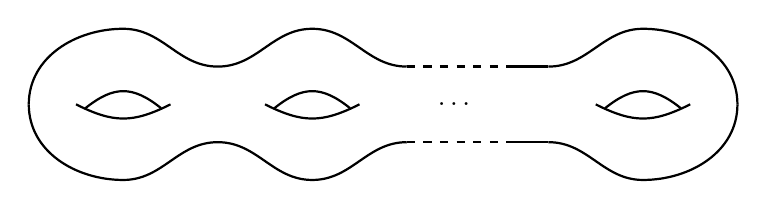
\begin{tikzpicture}[scale=1.2, line width=0.8pt]

    % Definizione corretta del comando \buco con 2 argomenti
    \def\buco#1#2{%
        \draw (#1-0.5, #2) .. controls (#1-0.1, #2-0.2) and (#1+0.1, #2-0.2) .. (#1+0.5, #2);%
        \draw (#1-0.4, #2-0.04) .. controls (#1-0.1, #2+0.2) and (#1+0.1, #2+0.2) .. (#1+0.4, #2-0.04);%
    }

    % -- Parte Sinistra: Sigma_{g-1} senza un punto (U) --
    \draw (-4, 0) to[out=90, in=180] (-3, 0.8)
                  to[out=0, in=180] (-2, 0.4)
                  to[out=0, in=180] (-1, 0.8)
                  to[out=0, in=180] (0, 0.4); % Collo aperto a destra

    \draw (-4, 0) to[out=-90, in=180] (-3, -0.8)
                  to[out=0, in=180] (-2, -0.4)
                  to[out=0, in=180] (-1, -0.8)
                  to[out=0, in=180] (0, -0.4); % Collo aperto a destra

    \buco{-3}{0}
    \buco{-1}{0}

    % -- Parte Centrale: Tratteggio e sovrapposizione --
    \draw[dashed] (0, 0.4) -- (1.13, 0.4);
    \draw[dashed] (0, -0.4) -- (1.13, -0.4);


    % Puntini di sospensione per il genere generico
    \node at (0.5, 0) {$\dots$};

    % -- Parte Destra: Toro bucato (V) --
    \draw (1.13, 0.4) -- (1.5, 0.4);
    \draw (1.13, -0.4) -- (1.5, -0.4);

    \draw (1.5, 0.4) to[out=0, in=180] (2.5, 0.8)
                   to[out=0, in=90] (3.5, 0);

    \draw (1.5, -0.4) to[out=0, in=180] (2.5, -0.8)
                    to[out=0, in=-90] (3.5, 0);

    \buco{2.5}{0}

\end{tikzpicture}
\end{equation*}
\caption{\label{fig:multitoro_normale}La superficie \(\Sigma_{g}\)}
\end{figure}


\begin{figure}
\begin{equation*}
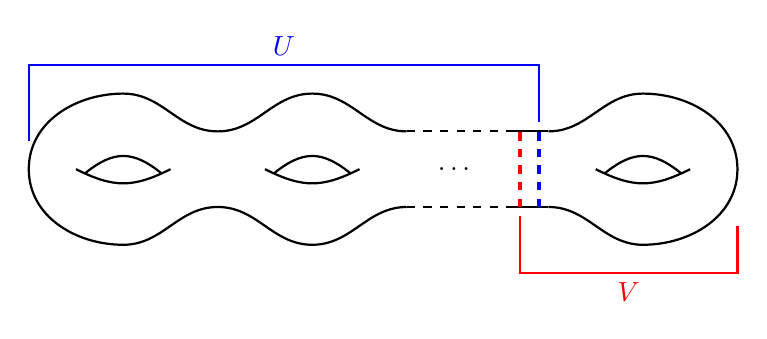
\begin{tikzpicture}[scale=1.2, line width=0.8pt]

    % Definizione corretta del comando \buco con 2 argomenti
    \def\buco#1#2{%
        \draw (#1-0.5, #2) .. controls (#1-0.1, #2-0.2) and (#1+0.1, #2-0.2) .. (#1+0.5, #2);%
        \draw (#1-0.4, #2-0.04) .. controls (#1-0.1, #2+0.2) and (#1+0.1, #2+0.2) .. (#1+0.4, #2-0.04);%
    }

    % -- Parte Sinistra: Sigma_{g-1} senza un punto (U) --
    \draw (-4, 0) to[out=90, in=180] (-3, 0.8)
                  to[out=0, in=180] (-2, 0.4)
                  to[out=0, in=180] (-1, 0.8)
                  to[out=0, in=180] (0, 0.4); % Collo aperto a destra

    \draw (-4, 0) to[out=-90, in=180] (-3, -0.8)
                  to[out=0, in=180] (-2, -0.4)
                  to[out=0, in=180] (-1, -0.8)
                  to[out=0, in=180] (0, -0.4); % Collo aperto a destra

    \buco{-3}{0}
    \buco{-1}{0}

    % -- Parte Centrale: Tratteggio e sovrapposizione --
    \draw[dashed] (0, 0.4) -- (1.13, 0.4);
    \draw[dashed] (0, -0.4) -- (1.13, -0.4);


    % Puntini di sospensione per il genere generico
    \node at (0.5, 0) {$\dots$};

    % -- Parte Destra: Toro bucato (V) --
    \draw (1.13, 0.4) -- (1.5, 0.4);
    \draw (1.13, -0.4) -- (1.5, -0.4);

    \draw (1.5, 0.4) to[out=0, in=180] (2.5, 0.8)
                   to[out=0, in=90] (3.5, 0);

    \draw (1.5, -0.4) to[out=0, in=180] (2.5, -0.8)
                    to[out=0, in=-90] (3.5, 0);

    \buco{2.5}{0}

    \draw[red, line width=1.2pt, dashed] (1.2, -0.4) -- (1.2, 0.4);
    \draw[red] (1.2, -0.5) -- (1.2, -1.1) -- (3.5, -1.1) -- (3.5, -0.6);
    \node at (2.35,-1.3) {\textcolor{red}{\(V\)}};

    \draw[blue, line width=1.2pt, dashed] (1.4, -0.4) -- (1.4, 0.4);
    \draw[blue] (1.4, 0.5) -- (1.4, 1.1) -- (-4, 1.1) -- (-4, 0.3);
    \node at (-1.3,1.3) {\textcolor{blue}{\(U\)}};
\end{tikzpicture}
\end{equation*}
\caption{\label{fig:multitoro_UeV}Gli insiemi \(U\) e \(V\)}
\end{figure}

\begin{figure}
\begin{equation*}
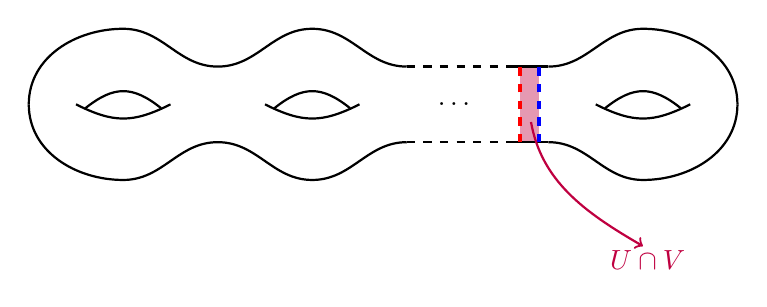
\begin{tikzpicture}[scale=1.2, line width=0.8pt]

    \fill[color=purple!40] (1.2, -0.4) rectangle (1.4, 0.4);

%    \fill[pattern=north west lines, pattern color=red] (1.2, -0.4) rectangle (1.4, 0.4);

    % Definizione corretta del comando \buco con 2 argomenti
    \def\buco#1#2{%
        \draw (#1-0.5, #2) .. controls (#1-0.1, #2-0.2) and (#1+0.1, #2-0.2) .. (#1+0.5, #2);%
        \draw (#1-0.4, #2-0.04) .. controls (#1-0.1, #2+0.2) and (#1+0.1, #2+0.2) .. (#1+0.4, #2-0.04);%
    }

    % -- Parte Sinistra: Sigma_{g-1} senza un punto (U) --
    \draw (-4, 0) to[out=90, in=180] (-3, 0.8)
                  to[out=0, in=180] (-2, 0.4)
                  to[out=0, in=180] (-1, 0.8)
                  to[out=0, in=180] (0, 0.4); % Collo aperto a destra

    \draw (-4, 0) to[out=-90, in=180] (-3, -0.8)
                  to[out=0, in=180] (-2, -0.4)
                  to[out=0, in=180] (-1, -0.8)
                  to[out=0, in=180] (0, -0.4); % Collo aperto a destra

    \buco{-3}{0}
    \buco{-1}{0}

    % -- Parte Centrale: Tratteggio e sovrapposizione --
    \draw[dashed] (0, 0.4) -- (1.13, 0.4);
    \draw[dashed] (0, -0.4) -- (1.13, -0.4);


    % Puntini di sospensione per il genere generico
    \node at (0.5, 0) {$\dots$};

    % -- Parte Destra: Toro bucato (V) --
    \draw (1.13, 0.4) -- (1.5, 0.4);
    \draw (1.13, -0.4) -- (1.5, -0.4);

    \draw (1.5, 0.4) to[out=0, in=180] (2.5, 0.8)
                   to[out=0, in=90] (3.5, 0);

    \draw (1.5, -0.4) to[out=0, in=180] (2.5, -0.8)
                    to[out=0, in=-90] (3.5, 0);

    \buco{2.5}{0}

    \draw[red, line width=1.2pt, dashed] (1.2, -0.4) -- (1.2, 0.4);

    \draw[blue, line width=1.2pt, dashed] (1.4, -0.4) -- (1.4, 0.4);

% 2. ETICHETTA E FRECCIA U CAP V:
    % Definiamo un nodo per l'etichetta posizionato in basso a destra
    \node at (2.55, -1.65) {\textcolor{purple}{$U \cap V$}};

    % Disegniamo la freccia. 'shorten >=' fa fermare la punta poco prima del target.
    % Usiamo 'to[out=..., in=...]' per una freccia curva più elegante.
    \draw[<-, thick, purple, shorten >= 3pt] (2.5, -1.5) to[out=150, in=-80] (1.3, -0.1);
\end{tikzpicture}
\end{equation*}
\caption{\label{fig:multitoro_UcapV}L'insieme \(U\cap V\)}
\end{figure}
\subsection{Caratterizzazione forme esatte di grado massimo a supporto compatto su varietà orientabile connessa}
\label{sec:org313a48c}
\begin{prop}
Sia \(M\) una \href{20250113115909-struttura_differenziabile.org}{varietà differenziabile} \hyperref[sec:org92acb5c]{orientabile}, \href{20250103165325-spazio_topologico_connesso.org}{connessa}. Allora una \hyperref[sec:orgcd9945f]{\(n\)-forma differenziale \(\omega \in A^{n}_{\text{c}}(M)\)} a \href{20251229110021-forma_differenziale_a_supporto_compatto.org}{supporto compatto} è \hyperref[sec:orgd00f880]{esatta} sse l'\hyperref[sec:org490b1d0]{integrale}
\begin{equation*}
\int_{M} \omega = 0.
\end{equation*}
\end{prop}
\begin{proof}
(\(\Rightarrow\)): per il \hyperref[sec:orge60a437]{Teorema di Stokes}.

(\(\Leftarrow\)): Per la \href{20251229114152-dualita_di_poincare.org}{Dualità di Poincaré} (e \hyperref[sec:org1dab48c]{Coomologia in dimensione massima}), si ha che \hyperref[sec:orgfc0ec93]{\(H^{n}_{\text{c}}(M)\)} ha dimensione 1. Pertanto:
\begin{align*}
\int_{M}: H^{n}_{\text{c}}(M) &\longrightarrow \R\\
[\omega] &\longmapsto \int_{M}\omega
\end{align*}
è un isomorfismo. Infatti
\begin{enumerate}
\item \(\int_{M}\) è lineare;
\item sia dominio che codominio hanno dimensione 1;
\item siccome \(H^{n}_{\text{c}} \cong \R\), allora \(H^{n}_{\text{c}} = \langle [\omega_{M}]\rangle\); \href{20251117121206-coomologia_in_dimensione_massima.org}{posso sempre scegliere} \(\omega_{M}\) tale che \(\int_{M} \omega_{M} = 1\), e pertanto \(\int_{M} \omega_{M} \neq 0\).
\end{enumerate}

Quindi, se \(\int_{M} \omega = 0\) allora \([\omega]= 0\) in \(H^{n}(M)\), ovvero \(\omega\) è esatta.
\end{proof}
\subsection{Funzione Propria}
\label{sec:orgf644f4d}
Siano \(X, Y\) \href{20250103145124-topologia.org}{spazi topologici}, \(F:X \longrightarrow Y\) \href{20250103103252-funzione_continua.org}{funzione continua}.

\begin{definizione}
\(F\) si dice \textbf{\textbf{propria}} se per ogni \(K \subseteq Y\) \href{20250103163701-spazio_topologico_compatto.org}{compatto}, la \href{20250202190147-immagine_punto_a_punto_di_due_classi.org}{retroimmagine} \(F^{-1}(K) \subseteq X\) è \href{20250103163701-spazio_topologico_compatto.org}{compatto}.
\end{definizione}
\subsection{Grado di una funzione propria tra varietà differenziabili}
\label{sec:org0e627c8}
\subsection{Teorema di Sard}
\label{sec:org687b9e8}
\subsection{Teorema del Grado}
\label{sec:orgcea54b7}
\end{document}
